\documentclass[12pt]{report}

%%%%%%%%%%%%%%%%%%%%%%%%%%%%%%%%%
% PACKAGE IMPORTS
%%%%%%%%%%%%%%%%%%%%%%%%%%%%%%%%%


\usepackage[tmargin=2cm,rmargin=1in,lmargin=1in,margin=0.85in,bmargin=2cm,footskip=.2in]{geometry}
\usepackage{amsmath,amsfonts,amsthm,amssymb}
\usepackage[varbb]{newpxmath}
\usepackage{xfrac}
\usepackage[makeroom]{cancel}
\usepackage{mathtools}
\usepackage{bookmark}
\usepackage{enumitem}
\usepackage{hyperref,theoremref}
\hypersetup{
	pdftitle={Assignment},
	colorlinks=true, linkcolor=doc!90,
	bookmarksnumbered=true,
	bookmarksopen=true
}
\usepackage[most,many,breakable]{tcolorbox}
\usepackage{xcolor}
\usepackage{varwidth}
\usepackage{varwidth}
\usepackage{etoolbox}
%\usepackage{authblk}
\usepackage{nameref}
\usepackage{multicol,array}
\usepackage{tikz-cd}
\usepackage[ruled,vlined,linesnumbered]{algorithm2e}
\usepackage{comment} % enables the use of multi-line comments (\ifx \fi) 
\usepackage{import}
\usepackage{xifthen}
\usepackage{pdfpages}
\usepackage{transparent}
\usepackage{physics}
\usepackage{caption}
\usepackage{siunitx}
\usepackage[version=4]{mhchem}
\usepackage{modiagram}
\usepackage{booktabs}

\captionsetup{textfont={footnotesize}, labelfont=bf}

\newcommand\mycommfont[1]{\footnotesize\ttfamily\textcolor{blue}{#1}}
\SetCommentSty{mycommfont}
\newcommand{\incfig}[1]{%
    \def\svgwidth{\columnwidth}
    \import{./figures/}{#1.pdf_tex}
}

\usepackage{tikzsymbols}
\renewcommand\qedsymbol{$\Laughey$}

%%%%%%%%%%%%%%%%%%%%%%%%%%%%%%
% DEFAULT FONT
%%%%%%%%%%%%%%%%%%%%%%%%%%%%%%

\usepackage{anyfontsize}
\usepackage{tgtermes}
\usepackage[T1]{fontenc}

%%%%%%%%%%%%%%%%%%%%%%%%%%%%%%
% SELF MADE COLORS
%%%%%%%%%%%%%%%%%%%%%%%%%%%%%%



\definecolor{myg}{RGB}{56, 140, 70}
\definecolor{myb}{RGB}{45, 111, 177}
\definecolor{myr}{RGB}{199, 68, 64}
\definecolor{mytheorembg}{HTML}{F2F2F9}
\definecolor{mytheoremfr}{HTML}{00007B}
\definecolor{mylenmabg}{HTML}{FFFAF8}
\definecolor{mylenmafr}{HTML}{983b0f}
\definecolor{mypropbg}{HTML}{f2fbfc}
\definecolor{mypropfr}{HTML}{191971}
\definecolor{myexamplebg}{HTML}{F2FBF8}
\definecolor{myexamplefr}{HTML}{88D6D1}
\definecolor{myexampleti}{HTML}{2A7F7F}
\definecolor{mydefinitbg}{HTML}{E5E5FF}
\definecolor{mydefinitfr}{HTML}{3F3FA3}
\definecolor{notesgreen}{RGB}{0,162,0}
\definecolor{myp}{RGB}{197, 92, 212}
\definecolor{mygr}{HTML}{2C3338}
\definecolor{myred}{RGB}{127,0,0}
\definecolor{myyellow}{RGB}{169,121,69}


%%%%%%%%%%%%%%%%%%%%%%%%%%%%
% TCOLORBOX SETUPS
%%%%%%%%%%%%%%%%%%%%%%%%%%%%

\setlength{\parindent}{1cm}
%================================
% THEOREM BOX
%================================

\tcbuselibrary{theorems,skins,hooks}
\newtcbtheorem[number within=section]{Theorem}{Theorem}
{%
	enhanced,
	breakable,
	colback = mytheorembg,
	frame hidden,
	boxrule = 0sp,
	borderline west = {2pt}{0pt}{mytheoremfr},
	sharp corners,
	detach title,
	before upper = \tcbtitle\par\smallskip,
	coltitle = mytheoremfr,
	fonttitle = \sffamily,
	description font = \mdseries,
	% separator sign none,
	segmentation style={solid, mytheoremfr},
}
{th}

\tcbuselibrary{theorems,skins,hooks}
\newtcbtheorem[number within=chapter]{theorem}{Theorem}
{%
	enhanced,
	breakable,
	colback = mytheorembg,
	frame hidden,
	boxrule = 0sp,
	borderline west = {2pt}{0pt}{mytheoremfr},
	sharp corners,
	detach title,
	before upper = \tcbtitle\par\smallskip,
	coltitle = mytheoremfr,
	fonttitle = \sffamily,
	description font = \mdseries,
	separator sign none,
	segmentation style={solid, mytheoremfr},
}
{th}


\tcbuselibrary{theorems,skins,hooks}
\newtcolorbox{Theoremcon}
{%
	enhanced
	,breakable
	,colback = mytheorembg
	,frame hidden
	,boxrule = 0sp
	,borderline west = {2pt}{0pt}{mytheoremfr}
	,sharp corners
	,description font = \mdseries
	,separator sign none
}

%================================
% Corollery
%================================
\tcbuselibrary{theorems,skins,hooks}
\newtcbtheorem[number within=section]{Corollary}{Corollary}
{%
	enhanced
	,breakable
	,colback = myp!10
	,frame hidden
	,boxrule = 0sp
	,borderline west = {2pt}{0pt}{myp!85!black}
	,sharp corners
	,detach title
	,before upper = \tcbtitle\par\smallskip
	,coltitle = myp!85!black
	,fonttitle = \sffamily
	,description font = \mdseries
	,separator sign none
	,segmentation style={solid, myp!85!black}
}
{th}
\tcbuselibrary{theorems,skins,hooks}
\newtcbtheorem[number within=chapter]{corollary}{Corollary}
{%
	enhanced
	,breakable
	,colback = myp!10
	,frame hidden
	,boxrule = 0sp
	,borderline west = {2pt}{0pt}{myp!85!black}
	,sharp corners
	,detach title
	,before upper = \tcbtitle\par\smallskip
	,coltitle = myp!85!black
	,fonttitle = \sffamily
	,description font = \mdseries
	,separator sign none
	,segmentation style={solid, myp!85!black}
}
{th}


%================================
% LENMA
%================================

\tcbuselibrary{theorems,skins,hooks}
\newtcbtheorem[number within=section]{Lenma}{Lenma}
{%
	enhanced,
	breakable,
	colback = mylenmabg,
	frame hidden,
	boxrule = 0sp,
	borderline west = {2pt}{0pt}{mylenmafr},
	sharp corners,
	detach title,
	before upper = \tcbtitle\par\smallskip,
	coltitle = mylenmafr,
	fonttitle = \bfseries\sffamily,
	description font = \mdseries,
	separator sign none,
	segmentation style={solid, mylenmafr},
}
{th}

\tcbuselibrary{theorems,skins,hooks}
\newtcbtheorem[number within=chapter]{lenma}{Lenma}
{%
	enhanced,
	breakable,
	colback = mylenmabg,
	frame hidden,
	boxrule = 0sp,
	borderline west = {2pt}{0pt}{mylenmafr},
	sharp corners,
	detach title,
	before upper = \tcbtitle\par\smallskip,
	coltitle = mylenmafr,
	fonttitle = \bfseries\sffamily,
	description font = \mdseries,
	separator sign none,
	segmentation style={solid, mylenmafr},
}
{th}


%================================
% PROPOSITION
%================================

\tcbuselibrary{theorems,skins,hooks}
\newtcbtheorem[number within=section]{Prop}{Proposition}
{%
	enhanced,
	breakable,
	colback = mypropbg,
	frame hidden,
	boxrule = 0sp,
	borderline west = {2pt}{0pt}{mypropfr},
	sharp corners,
	detach title,
	before upper = \tcbtitle\par\smallskip,
	coltitle = mypropfr,
	fonttitle = \bfseries\sffamily,
	description font = \mdseries,
	separator sign none,
	segmentation style={solid, mypropfr},
}
{th}

\tcbuselibrary{theorems,skins,hooks}
\newtcbtheorem[number within=chapter]{prop}{Proposition}
{%
	enhanced,
	breakable,
	colback = mypropbg,
	frame hidden,
	boxrule = 0sp,
	borderline west = {2pt}{0pt}{mypropfr},
	sharp corners,
	detach title,
	before upper = \tcbtitle\par\smallskip,
	coltitle = mypropfr,
	fonttitle = \bfseries\sffamily,
	description font = \mdseries,
	separator sign none,
	segmentation style={solid, mypropfr},
}
{th}


%================================
% CLAIM
%================================

\tcbuselibrary{theorems,skins,hooks}
\newtcbtheorem[number within=section]{claim}{Claim}
{%
	enhanced
	,breakable
	,colback = myg!10
	,frame hidden
	,boxrule = 0sp
	,borderline west = {2pt}{0pt}{myg}
	,sharp corners
	,detach title
	,before upper = \tcbtitle\par\smallskip
	,coltitle = myg!85!black
	,fonttitle = \bfseries\sffamily
	,description font = \mdseries
	,separator sign none
	,segmentation style={solid, myg!85!black}
}
{th}




%================================
% EXAMPLE BOX
%================================

\newtcbtheorem[number within=section]{Example}{Example}
{%
	colback = myexamplebg
	,breakable
	,colframe = myexamplefr
	,coltitle = myexampleti
	,boxrule = 1pt
	,sharp corners
	,detach title
	,before upper=\tcbtitle\par\smallskip
	,fonttitle = \bfseries
	,description font = \mdseries
	,separator sign none
	,description delimiters parenthesis
}
{ex}

\newtcbtheorem[number within=chapter]{example}{Example}
{%
	colback = myexamplebg
	,breakable
	,colframe = myexamplefr
	,coltitle = myexampleti
	,boxrule = 1pt
	,sharp corners
	,detach title
	,before upper=\tcbtitle\par\smallskip
	,fonttitle = \bfseries
	,description font = \mdseries
	,separator sign none
	,description delimiters parenthesis
}
{ex}

%================================
% DEFINITION BOX
%================================

\newtcbtheorem[number within=section]{Definition}{Definition}{enhanced,
	before skip=2mm,after skip=2mm, colback=red!5,colframe=red!80!black,boxrule=0.5mm,
	attach boxed title to top left={xshift=1cm,yshift*=1mm-\tcboxedtitleheight}, varwidth boxed title*=-3cm,
	boxed title style={frame code={
					\path[fill=tcbcolback]
					([yshift=-1mm,xshift=-1mm]frame.north west)
					arc[start angle=0,end angle=180,radius=1mm]
					([yshift=-1mm,xshift=1mm]frame.north east)
					arc[start angle=180,end angle=0,radius=1mm];
					\path[left color=tcbcolback!60!black,right color=tcbcolback!60!black,
						middle color=tcbcolback!80!black]
					([xshift=-2mm]frame.north west) -- ([xshift=2mm]frame.north east)
					[rounded corners=1mm]-- ([xshift=1mm,yshift=-1mm]frame.north east)
					-- (frame.south east) -- (frame.south west)
					-- ([xshift=-1mm,yshift=-1mm]frame.north west)
					[sharp corners]-- cycle;
				},interior engine=empty,
		},
	fonttitle=\bfseries,
	title={#2},#1}{def}
\newtcbtheorem[number within=chapter]{definition}{Definition}{enhanced,
	before skip=2mm,after skip=2mm, colback=red!5,colframe=red!80!black,boxrule=0.5mm,
	attach boxed title to top left={xshift=1cm,yshift*=1mm-\tcboxedtitleheight}, varwidth boxed title*=-3cm,
	boxed title style={frame code={
					\path[fill=tcbcolback]
					([yshift=-1mm,xshift=-1mm]frame.north west)
					arc[start angle=0,end angle=180,radius=1mm]
					([yshift=-1mm,xshift=1mm]frame.north east)
					arc[start angle=180,end angle=0,radius=1mm];
					\path[left color=tcbcolback!60!black,right color=tcbcolback!60!black,
						middle color=tcbcolback!80!black]
					([xshift=-2mm]frame.north west) -- ([xshift=2mm]frame.north east)
					[rounded corners=1mm]-- ([xshift=1mm,yshift=-1mm]frame.north east)
					-- (frame.south east) -- (frame.south west)
					-- ([xshift=-1mm,yshift=-1mm]frame.north west)
					[sharp corners]-- cycle;
				},interior engine=empty,
		},
	fonttitle=\bfseries,
	title={#2},#1}{def}



%================================
% EXERCISE BOX
%================================

\makeatletter
\newtcbtheorem{question}{}{enhanced,
	breakable,
	colback=white,
	colframe=myb!80!black,
	attach boxed title to top left={yshift*=-\tcboxedtitleheight},
	fonttitle=\bfseries,
	title={#2},
	boxed title size=title,
	boxed title style={%
			sharp corners,
			rounded corners=northwest,
			colback=tcbcolframe,
			boxrule=0pt,
		},
	underlay boxed title={%
			\path[fill=tcbcolframe] (title.south west)--(title.south east)
			to[out=0, in=180] ([xshift=5mm]title.east)--
			(title.center-|frame.east)
			[rounded corners=\kvtcb@arc] |-
			(frame.north) -| cycle;
		},
	#1
}{def}
\makeatother

%================================
% SOLUTION BOX
%================================

\makeatletter
\newtcolorbox{solution}{enhanced,
	breakable,
	colback=white,
	colframe=myg!80!black,
	attach boxed title to top left={yshift*=-\tcboxedtitleheight},
	title=Solution,
	boxed title size=title,
	boxed title style={%
			sharp corners,
			rounded corners=northwest,
			colback=tcbcolframe,
			boxrule=0pt,
		},
	underlay boxed title={%
			\path[fill=tcbcolframe] (title.south west)--(title.south east)
			to[out=0, in=180] ([xshift=5mm]title.east)--
			(title.center-|frame.east)
			[rounded corners=\kvtcb@arc] |-
			(frame.north) -| cycle;
		},
}
\makeatother

%================================
% Question BOX
%================================

\makeatletter
\newtcbtheorem{qstion}{Question}{enhanced,
	breakable,
	colback=white,
	colframe=mygr,
	attach boxed title to top left={yshift*=-\tcboxedtitleheight},
	fonttitle=\bfseries,
	title={#2},
	boxed title size=title,
	boxed title style={%
			sharp corners,
			rounded corners=northwest,
			colback=tcbcolframe,
			boxrule=0pt,
		},
	underlay boxed title={%
			\path[fill=tcbcolframe] (title.south west)--(title.south east)
			to[out=0, in=180] ([xshift=5mm]title.east)--
			(title.center-|frame.east)
			[rounded corners=\kvtcb@arc] |-
			(frame.north) -| cycle;
		},
	#1
}{def}
\makeatother

\makeatletter
\newtcolorbox{wconc}[1]{
	breakable,
	enhanced,
	colback=white,
	colframe=myr,
	arc=0pt,
	title={#1},
	outer arc=0pt,
	fonttitle=\bfseries\large,
	colbacktitle=myr,
	attach boxed title to top left={},
	boxed title style={
			enhanced,
			skin=enhancedfirst jigsaw,
			arc=3pt,
			bottom=0pt,
			interior style={fill=myr}
		},
}
\makeatother

% \newtcbtheorem[number within=chapter]{wconc}{Wrong Concept}{
% 	breakable,
% 	enhanced,
% 	colback=white,
% 	colframe=myr,
% 	arc=0pt,
% 	outer arc=0pt,
% 	fonttitle=\bfseries\sffamily\large,
% 	colbacktitle=myr,
% 	attach boxed title to top left={},
% 	boxed title style={
% 			enhanced,
% 			skin=enhancedfirst jigsaw,
% 			arc=3pt,
% 			bottom=0pt,
% 			interior style={fill=myr}
% 		},
% 	#1
% }{def}



%================================
% NOTE BOX
%================================

\usetikzlibrary{arrows,calc,shadows.blur,positioning,shapes,shapes.multipart}
\tcbuselibrary{skins}
\newtcolorbox{note}[1][]{%
	enhanced jigsaw,
	colback=gray!20!white,%
	colframe=gray!80!black,
	size=small,
	boxrule=1pt,
	title=\textbf{Note},
	halign title=flush center,
	coltitle=black,
	breakable,
	drop shadow=black!50!white,
	attach boxed title to top left={xshift=1cm,yshift=-\tcboxedtitleheight/2,yshifttext=-\tcboxedtitleheight/2},
	minipage boxed title=1.5cm,
	boxed title style={%
			colback=white,
			size=fbox,
			boxrule=1pt,
			boxsep=2pt,
			underlay={%
					\coordinate (dotA) at ($(interior.west) + (-0.5pt,-0.5pt)$);
					\coordinate (dotB) at ($(interior.east) + (0.5pt,-0.5pt)$);
					\begin{scope}
						\clip (interior.north west) rectangle ([xshift=3ex]interior.east);
						\filldraw [white, blur shadow={shadow opacity=60, shadow yshift=-.75ex}, rounded corners=2pt] (interior.north west) rectangle (interior.south east);
					\end{scope}
					\begin{scope}[gray!80!black]
						\fill (dotA) circle (2pt);
						\fill (dotB) circle (2pt);
					\end{scope}
				},
		},
	#1,
}

%%%%%%%%%%%%%%%%%%%%%%%%%%%%%%
% SELF MADE COMMANDS
%%%%%%%%%%%%%%%%%%%%%%%%%%%%%%


\newcommand{\thm}[2]{\begin{Theorem}{#1}{}#2\end{Theorem}}
\newcommand{\cor}[2]{\begin{Corollary}{#1}{}#2\end{Corollary}}
\newcommand{\mlenma}[2]{\begin{Lenma}{#1}{}#2\end{Lenma}}
\newcommand{\mprop}[2]{\begin{Prop}{#1}{}#2\end{Prop}}
\newcommand{\clm}[3]{\begin{claim}{#1}{#2}#3\end{claim}}
\newcommand{\wc}[2]{\begin{wconc}{#1}{}\setlength{\parindent}{1cm}#2\end{wconc}}
\newcommand{\thmcon}[1]{\begin{Theoremcon}{#1}\end{Theoremcon}}
\newcommand{\ex}[2]{\begin{Example}{#1}{}#2\end{Example}}
\newcommand{\dfn}[2]{\begin{Definition}[colbacktitle=red!75!black]{#1}{}#2\end{Definition}}
\newcommand{\dfnc}[2]{\begin{definition}[colbacktitle=red!75!black]{#1}{}#2\end{definition}}
\newcommand{\qs}[2]{\begin{question}{#1}{}#2\end{question}}
\newcommand{\pf}[2]{\begin{myproof}[#1]#2\end{myproof}}
\newcommand{\nt}[1]{\begin{note}\itshape #1\end{note}}

\newcommand*\circled[1]{\tikz[baseline=(char.base)]{
		\node[shape=circle,draw,inner sep=1pt] (char) {#1};}}
\newcommand\getcurrentref[1]{%
	\ifnumequal{\value{#1}}{0}
	{??}
	{\the\value{#1}}%
}
\newcommand{\getCurrentSectionNumber}{\getcurrentref{section}}
\newenvironment{myproof}[1][\proofname]{%
	\proof[\bfseries #1: ]%
}{\endproof}
\newcounter{mylabelcounter}

\makeatletter
\newcommand{\setword}[2]{%
	\phantomsection
	#1\def\@currentlabel{\unexpanded{#1}}\label{#2}%
}
\makeatother




\tikzset{
	symbol/.style={
			draw=none,
			every to/.append style={
					edge node={node [sloped, allow upside down, auto=false]{$#1$}}}
		}
}



%%%%%%%%%%%%%%%%%%%%%%%%%%%%%%%%%%%%%%%%%%%
% TABLE OF CONTENTS
%%%%%%%%%%%%%%%%%%%%%%%%%%%%%%%%%%%%%%%%%%%

\newcounter{ContChapter}
\setcounter{ContChapter}{0}
\newcommand\showmycounter{\addtocounter{ContChapter}{1}}

\usepackage{tikz}
\definecolor{doc}{RGB}{0,60,110}
\usepackage{titletoc}
\contentsmargin{0cm}
\titlecontents{chapter}[3.7pc]
{\addvspace{30pt}%
	\begin{tikzpicture}[remember picture, overlay]%
		\draw[fill=doc!60,draw=doc!60] (-7,-.1) rectangle (-0.4,.5);%
		\pgftext[left,x=-3.5cm,y=0.2cm]{\color{white}\Large\sc\bfseries Chapter \showmycounter\ \thecontentslabel};%
	\end{tikzpicture}\color{doc!60}\large\sc\bfseries}%
{}
{}
{\;\titlerule\;\large\sc\bfseries Page \thecontentspage
	\begin{tikzpicture}[remember picture, overlay]
		\draw[fill=doc!60,draw=doc!60] (2pt,0) rectangle (4,0.1pt);
	\end{tikzpicture}}%

\titlecontents{section}[3.7pc]
{\addvspace{2pt}}
{\contentslabel[\thecontentslabel]{2pc}}
{}
{\hfill\small \thecontentspage}
[]

\titlecontents*{subsection}[3.7pc]
{\addvspace{-1pt}\small}
{}
{}
{\ --- \small\thecontentspage}
[ \textbullet\ ][]

%! Sembra che tu possa usare un qualsiasi tipo di sezione al posto di subsubsection o chapter ecc e funziona uguale, per cui se hai intenzione di modificare lo stile di quella sezione che poi ti va a sminchiare questo basta cambiarlo in un'altro che non userai.
\makeatletter
\renewcommand{\tableofcontents}{%
	\subsubsection*{%
	  \vspace*{-20\p@}%
	  \begin{tikzpicture}[remember picture, overlay]%
		  \pgftext[right,x=15cm,y=0.2cm]{\color{doc!60}\Huge\bfseries \contentsname};%
		  \draw[fill=doc!60,draw=doc!60] (13,-.75) rectangle (20,1);%
		  \clip (13,-.75) rectangle (20,1);
		  \pgftext[right,x=15cm,y=0.2cm]{\color{white}\Huge\bfseries \contentsname};%
	  \end{tikzpicture}}
	\@starttoc{toc}}
\makeatother


%%%%%%%%%%%%%%%%%%%%%%%%%%%%%%%%%%%%%%%%%%%
% SECTION MODIFICATION
%%%%%%%%%%%%%%%%%%%%%%%%%%%%%%%%%%%%%%%%%%%

\usepackage[explicit]{titlesec}
\usepackage{varwidth}

%------------------------------------------
% CHAPTERS
%------------------------------------------

\titleformat{\chapter}[display]
  {\normalfont\Huge\bfseries}
  {
	\begin{tikzpicture}[remember picture, overlay]%
		\pgftext[right,x=15cm,y=0.2cm]{\color{doc!60}\usefont{T1}{pnc}{b}{n}\fontsize{50}{60}\selectfont\bfseries \thechapter};%
		\draw[fill=doc!60,draw=doc!60] (13,-.75) rectangle (20,1);%
		\clip (13,-.75) rectangle (20,1);
		\pgftext[right,x=15cm,y=0.2cm]{\color{white}\usefont{T1}{pnc}{b}{n}\fontsize{50}{60}\selectfont\bfseries \thechapter};%
	\end{tikzpicture}
  }
  {20pt}
  {
	\filcenter
	\begin{tikzpicture}
		\node[fill=gray!40] () 
		{
			\begin{varwidth}{18cm}
				\centering
				\Huge\bfseries #1
			\end{varwidth}
		};
	\end{tikzpicture}
  }
  {}

%------------------------------------------
% SECTIONS
%------------------------------------------

\titleformat{\section}
 {\normalfont\Large\bfseries}
 {}
 {0pt}
 {
	\begin{tikzpicture}[overlay]
		\node[fill=doc!60, minimum height=1cm] (a) {\Large\bfseries \color{white} \thesection};
		\node[fill=gray!40, right= 0pt of a.east, minimum height=1cm] (b) {\Large\bfseries \textcolor{black}{}#1};
	\end{tikzpicture}
 }

%------------------------------------------
% SUBSECTIONS
%------------------------------------------

\titleformat{\subsection}
 [hang]
 {\large\bfseries}
 {}
 {0pt}
 {
	\begin{tikzpicture}
 		\node[fill=gray!40,draw=doc!60, rounded corners=1mm,text depth=0.2ex,line width=2pt,anchor=west](a){\large\bfseries \textcolor{black}{}#1};
 		\coordinate (b) at (\textwidth-2em,0);
 		\draw[color=doc!60, line width=2pt] (a)--(b);
	\end{tikzpicture}
 }

%%%%%%%%%%%%%%%%%%%%%%%%%%%%%%%%%%%%%%%%%%%
% COMAND FOR REFERENCES
%%%%%%%%%%%%%%%%%%%%%%%%%%%%%%%%%%%%%%%%%%%

\newcommand{\figref}[1]{Fig. (\ref{#1})}
\newcommand{\tabref}[1]{Tab. (\ref{#1})}
\renewcommand{\eqref}[1]{Eq. (\ref{#1})}

\title{\Huge{Quantum Computing}\\Notes of the course}
\author{\huge{Luca Leoni}}
\date{}

\begin{document}
    \maketitle

    \tableofcontents

    \chapter{Introduction to quantum computations}
    \section{Postulates of quantum mechanics}

The course has the aim of introducing the follower to the working principles of quantum computing and how they work on a fundamental physical and mathematical level. Therefore, will come to the mind of the reader that all the theory ahead of us will rely on quantum mechanical principles that we will need to introduce first. This will be useful also to the experienced reader since a refresh can is always good, and also because we may want to restate the fundamental of quantum mechanics specifically for application to quantum calculators.

Quantum mechanics(QM) is the modern fundamental theory that describes reality and relies on a series of assumptions, or postulates, that allow us to describe the physical systems. There is not a standard version of the postulates, can vary in numbers, but we are going to use the description of QM that uses three postulates to define: states, evolution and mesuraments.

\subsection{Postulate 1}

\dfn{States}{
    The set containing the possible states of the system is a Hilbert space $\mathcal{H}$ and of the vectors $\ket{\psi} \in \mathcal{H}$ only the normalized ones can describe the real state of the system.
}

\noindent
This definition of the notion of state is really different from the simple coordinate couples of position and momenta $(\vb{r}, \vb{p})$ that we had in classical mechanics. In this situation the states are pure vectors inside a vector space that is the Hilbert space itself, meaning that all the properties known from linear algebra theory apply to them. In particular, we have the closure property of sum and multiplication with a scalar, or the presence of a scalar product $<\vdot,\vdot> : \mathcal{H}\otimes\mathcal{H} \to \mathbb{C}$. Those are all things that need to be present inside $\mathcal{H}$ to be an Hilbert space, and define those inside our restricted series of systems that describe quantum computer is simple. In fact, the main quantum computers rely on systems with a finite number of levels which posses a \textbf{finite dimensional} $\mathcal{H}$ which allow us to highly simplify all the computations thanks to the following 

\thm{}{If we have that $\dim \mathcal{H} = N$ then the space is holomorphic to $\mathbb{C}^{N}$.}

\noindent
That is a known fact indeed, but allow us to directly describe all the states of the system as complex vectors, along with the possible bases and the inner product. In fact, if we have a space with dimension $N$ we can write down directly an orthonormal base for the system as the canonical one and write whatever vector $\ket{\psi}$ as a superposition of those
\begin{align*}
    &\ket{i} = \begin{pmatrix}
        0\\
        \vdots\\
        1\\
        \vdots\\
        0\\
    \end{pmatrix}
    & \ket{\psi} = \sum_i \lambda_i \ket{i}.
\end{align*}
The other part is that we can imagine the inner product inside this space to be exactly the one of the complex space, having so that we can simply define it by first define the raw vectors as follows
\begin{align*}
    \bra{\phi} = \left(\ket{\phi}\right)^\dagger =  \begin{pmatrix}
        \alpha_0^*&
        \cdots&
        \alpha_i^*&
        \cdots&
        \alpha_N^*
    \end{pmatrix}.
\end{align*}
Then, we can use the normal algebra to define the following inner product inside the space
\begin{align*}
    \braket{\phi}{\psi} = \alpha_0^*\lambda_0 + \cdots + \alpha_N^*\lambda_N = \sum_i \alpha_i^*\lambda_i.
\end{align*}
Knowing it allow also to define to norm inside to space simply as $\norm{\psi}^2 = \braket{\psi}{\psi}$, which tells us that for a state to be normalized means that the following must be true, always
\begin{align}
    \braket{\psi}{\psi} = \sum_i \abs{\lambda_i}^2 = 1.
\end{align}
Which also show us how a state of a system doesn't care about the phase since even if I redefine it to be $\ket{\phi} = \exp(i\theta)\ket{\psi}$ will still be normalized, but one can also see how also observables are not touched.

We now have the full construction of the space we are going to use during our computations, and would be kind of interesting to use it to see how $\mathcal{H}$ will look like in some simple cases. In particular, we want to show how the states of a \textbf{qubit} are formed. The latter is non-other than a two level system, which so has $\dim\mathcal{H} = 2$, meaning that the base can be seen simply as

\begin{align*}
    &\ket{0} = \begin{pmatrix}
        1\\
        0
    \end{pmatrix},
    &\ket{1} = \begin{pmatrix}
        0\\
        1
    \end{pmatrix}.
\end{align*}
Which we will call as \textbf{computational base}, and all the state can be represented with them using a general linear combination that is normalized, so

\begin{align*}
    &\ket{\psi} = \begin{pmatrix}
        a\\
        b
    \end{pmatrix},
    & \abs{a}^2 + \abs{b}^2 = 1.
\end{align*}
This is effectively simple to use not only for its mathematical simplicity but also because a really simple geometric representation for those state can be used. In fact, one can see the following

\thm{}{
    A state $\ket{\psi}$ in a qubit can be represented, instead of using the $a$ and $b$ couple, using two angles $\theta \in [0, \pi]$ and $\phi \in [0, 2\pi]$ using the following form 
    \begin{equation}
        \ket{\psi} = \cos\left(\frac{\theta}{2}\right)\ket{0} + e^{i\phi}\sin\left(\frac{\theta}{2}\right)\ket{1}.
    \end{equation}
}
\pf{Proof}{
    Devo pensare alla dimostrazione.
}

\noindent
This allows us to see a state of the system as a unitary vector on a circumference, referenced by the angles and so the direction in which is pointing. This is indeed remarkable as we will see, since this anticipate the fact that every possible modification of a state is non-other than a rotation, as we will see.

In this construction we can also easily create systems composed by a series of qubit together, since the Hilbert space generated will be the tensor product of the single qubit ones as 
\begin{displaymath}
    \mathcal{H}_N = \mathcal{H} \otimes \cdots \otimes \mathcal{H} = \mathbb{C}^{2N}. 
\end{displaymath}
Since we are working with a known operation, that is the tensor product, we can also readily create basis functions for the new states by simply make the tensor product of the ones of the older states. For example, calling $\{\ket{0}_1, \ket{1}_1\}$ the base of the first qubit and $\{\ket{0}_2, \ket{1}_2\}$ the base of the second one can easily see that the base for the combined system will be 
\begin{displaymath}
    \{\ket{0}_1\ket{0}_2,\ket{0}_1\ket{1}_2, \ket{1}_1\ket{0}_2, \ket{1}_1\ket{1}_2 \}.
\end{displaymath}
Most of the time the subscripts are omited, having so that $\ket{0}_1\ket{0}_2 = \ket{00}$, but in this case the order in which you write the basis is important and needs to be remembered! The importance of order is also noticeable in the creation of a two-qubit state by using single qubit ones, if taken $\ket{\psi} = (a,b)$ and $\ket{\phi} = (cd)$ one can see how
\begin{align*}
    &\ket{\psi\phi} = \left(a\ket{0} + b\ket{1}\right)\otimes\left( c\ket{0} + d\ket{1} \right) \neq \left(c\ket{0} + d\ket{1}\right)\otimes\left( a\ket{0} + b\ket{1} \right) =  \ket{\phi\psi}.
\end{align*}
In fact the coefficients on the bases $\ket{01}$ and $\ket{10}$ are different, and the order here is important, so the states are different.

\nt{
    It's interesting to note how the number of basis elements increase a lot as the number of qubits are inserted inside the system. In particular, the dimension of the space scales as $2^N$. This is in contrast with what happens for the phase space in classical dynamics, where to describe a particle I need 6 coordinates and as the particle increase the number rise as $6N$. Basically the quantum systems become more complex much quicker and that hints us why is difficult simulate quantum systems on classical computers.
}

\subsection{Postulate 2}

\dfn{Evolution}{
    The evolution of a closed system can be represented using a unitary operator $\mathcal{U}(t_1, t_2)$ that acts on the state making it evolve in time as follows
    \begin{equation}
        \ket{\psi(t_2)} = \mathcal{U}(t_1, t_2)\ket{\psi(t_1)}.
    \end{equation}
}

\noindent
This is obviously a simplified version of the evolution postulate, which in reality should refer to the evolution of the state based on the Schr\"odinger equation(SE). In fact, we can also see how this principle can be derived directly from the latter. Therefore, let's start from the SE recalling its form
\begin{equation}
    \label{eq:SchEque}
    i\hbar\pdv{\ket{\psi(t)}}{t} = \hat{\mathcal{H}}\ket{\psi(t)},
\end{equation}
where, being in a closed system, the Hamiltonian will be time independent. Under those conditions we can easily integrate the equation finding out the following general form for the evolution of the system
\begin{equation}
    \ket{\psi(t)} = \exp\left( -i\frac{\hat{\mathcal{H}}}{\hbar}(t-t') \right)\ket{\psi(t')} = \mathcal{U}(t', t)\ket{\psi(t')}.
\end{equation}
In this way we have found out an analytic form for the evolution operator that we were describing. Also, one can actually see how since $\hat{\mathcal{H}}$ is assumed to be selfadjoint, $\hat{\mathcal{H}}^\dagger = \hat{\mathcal{H}}$, then the following holds true
\begin{align}
    \mathcal{U}^\dagger(t', t) = \mathcal{U}(t, t') = \mathcal{U}^{-1}.
\end{align}
Which is telling us that $\mathcal{U}$ is effectively unitary as required by the postulate, but not only that. In fact inside this construction we will also have that the operator $\mathcal{U}$ will be also \textbf{linear} and \textbf{invertible}, giving always rise to reversible operations.
\nt
{
    The properties of $\mathcal{U}$ of being linear and invertible are something that was not really present inside classical computers, in fact we will use that operator to manipulate qubits and every operation can be inverted. That didn't hold true for classical bits, where operations were often irreversible, or neither linear.
}

\subsection{Postulate 3}
When we will do it I will add it here.

\newpage
    \section{Quantum gates}

After recalling the postulates of QM we want to focus a little on the second one and understanding how we can manipulate the states of qubits using it. In particular, the second postulate tells us that the evolution of a state in time is described by a unitary operator $\mathcal{U}$. Normally that operator should have infinite dimensions, nevertheless the qubits posses a finite dimensional Hilbert space meaning that also the operators inside it can be associated to finite matrices. To understand this we can take a system composed by $N$ qubits, so that $\dim\mathcal{H} = 2^N$, the operator could then be described as follows
\begin{align}
    &\mathcal{U}: \mathbb{C}^{2N} \to \mathbb{C}^{2N}, &\mathcal{U} = \begin{pmatrix}
        a_{11} & \cdots & a_{2^{N}1}\\
        \vdots & \ddots & \vdots\\
        a_{12^N} & \cdots & a_{2^N2^N}
    \end{pmatrix}.
\end{align}
This representation is incredibly useful on a mathematical level, in fact manipulating a simple qubit state will become as doing a matrix multiplication. In particular, we know that the state of a qubit can be written generally as $\ket{\psi} = a\ket{0} + b\ket{1} = (a, b)$, so applying a generic state manipulation $\mathcal{U}$ will simply mean doing the following
\begin{equation}
    \label{eq:singleQuOp}
    \mathcal{U}\ket{\psi} = \begin{pmatrix}
        A & B\\
        C & D
    \end{pmatrix}\begin{pmatrix}
        a\\
        b
    \end{pmatrix} = 
    \begin{pmatrix}
        Aa + Bb\\
        Ca + Db
    \end{pmatrix} = \ket{\psi'}.
\end{equation}
This matrix operations are called \textbf{quantum gates}, and we want to try to unveil some possible interesting forms that they can have starting to understand how effectively a so-called \textbf{quantum circuits} works. In fact, a quantum circuits is non-other than a series of quantum gates acting on the available qubits in order to obtain a specific state in the end, as depicted in \figref{fig:FirstQC}.
\begin{figure}[b]
    \centering
    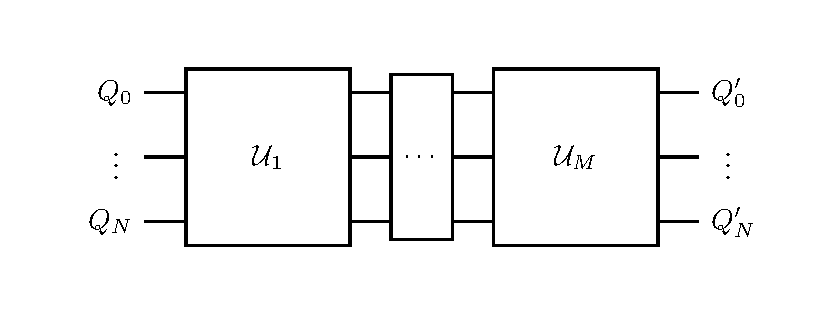
\includegraphics[width=0.91\textwidth]{Immagini/FirstQC.pdf}
    \caption{
        Sample image of a general quantum circuits where all the manipulations on the qubits are done using quantum gates, matrices, represented as blocks. 
    }
    \label{fig:FirstQC}
\end{figure}

Thus, what we want to do now is look deeper in the form that those gates can have, and try to identify some important operations that will follow us during the whole course. Therefore, I suggest to the reader (especially my future self) to look into them and try getting attune to their form and their actions on the qubits.

\subsection{Single qubit gates}

The first type of gates that we want to analyze are the one that acts a single qubits, which are also the simplest ones. As we have pointed out previously an operation of this type can be written as a matrix like in \eqref{eq:singleQuOp}. In particular, it's easy to understand that every $2\times 2$ matrix that is unitary satisfy the second postulate being a valid quantum gate for the manipulation of a qubit state. That let us have an infinite amount of possibilities for the operations that we can do on a single unit of information, setting another difference with the classical bits. In fact, a normal bit could be manipulated through the application of the identity operation, leaving as it is, or the NOT one, changing its state. So, not only the qubits allow for an infinite number of possible states to be represented using superposition, but also allow for an infinite number of operations to be done on it showing a clear superiority.

This simple observation has already shown to us that we have a lot of room in which we can move in order to work with qubit, and what we need to do now is to point out the most significant and important operations that are present inside this really large space. The first, thing that is important to point out is that we know how to generate every $2\times 2$ unitary matrix using four of them. Thus, mathematic has already given us a way to write down all the possible gates using a simple universal relation.
\thm{Universal single gate}
{
    Every quantum gate $\mathcal{U}$ can be associated to a rotation of the state on the Bloch sphere, and therefore can be written as
    \begin{equation}
        \mathcal{U} = e^{i\lambda\mathbb{1}}\exp\left( ia\vb{n}\vdot\vb*{\sigma} \right),
    \end{equation}
    where $\lambda, \alpha\in \mathbb{R}$, $\mathbb{1}$ is the identity matrix, $\vb{n}$ is an appropriate unitary vector, and $\vb*{\sigma}$ is a vector containing the three Pauli matrices.
    \begin{align}
        X = \mqty(\pmat{1}), \hspace{2cm} Y = \mqty(\pmat{2}), \hspace{2cm} Z = \mqty(\pmat{3}). 
    \end{align}
}
\noindent
This theorem tells us that only $4$ parameters are needed in order to define every possible gates, in fact the parameter $a$ is not really needed can be associated to the velocity of the rotation not really on the rotation itself. Therefore, we know how to write every possible operation, still the one that are interesting to us are limited, and so we will report them briefly discussing the form and the action of those specific gates.

\paragraph{NOT.} The NOT operation is the equivalent of the one in the classical case, meaning that the effect is the one of negating the current state. That can be easily done by recalling that the $0$ and $1$ of our quantum logic are the state $\ket{0}$ and $\ket{1}$, leading us to the possibility of constructing the truth table and matrix associated to this operation.

\begin{minipage}{0.45\textwidth}
    \centering
    \begin{tabular}{c|c}
        \textbf{IN} & \textbf{OUT}\\
        \midrule
        $\ket{0}$ & $\ket{1}$\\
        $\ket{1}$ & $\ket{0}$
    \end{tabular}
\end{minipage}
\begin{minipage}{0.45\textwidth}
    \centering
    \begin{equation}
        \text{NOT} = \scalebox{1.5}{$\begin{pmatrix}
            0 & 1\\
            1 & 0
        \end{pmatrix}$}
    \end{equation}.
\end{minipage}

\noindent
One can also notice that the final matrix obtained is exactly the $X$ Pauli matrix, with assure to us that is unitary since every one of them has the property $X^2 = Y^2 = Z^2 = \mathbb{1}$. This matrix is, in fact, drawn as $\bigoplus$ symbol inside circuits to recall that the $X$ matrix is getting used on a certain qubit.

\paragraph{Hadamart.} This is the first real quantum gate that was thought of, the idea is the one of creating superpositions of the normal states. This can be done really easily since the gate that we are interested in, and it's truth table, is

\begin{minipage}{0.45\textwidth}
    \centering
    \begin{tabular}{c|c}
        \textbf{IN} & \textbf{OUT}\\
        \midrule
        $\ket{0}$ & $\ket{+}$\\
        $\ket{1}$ & $\ket{-}$
    \end{tabular}
\end{minipage}
\begin{minipage}{0.45\textwidth}
    \centering
    \begin{equation}
        H = \scalebox{1.5}{$\frac{1}{\sqrt{2}}\begin{pmatrix}
            1 & 1\\
            1 & -1
        \end{pmatrix}$}
    \end{equation}.
\end{minipage}

\noindent
Where we shall recall how $\ket{\pm} = (\ket{0} \pm \ket{1})/\sqrt{2}$ are interesting states that forms the eigenvectors of the $X$ Pauli matrix, basically being the states in the $x$ direction on the Bloch sphere while the computational base is on the $z$ one. This gate has also really important properties that can be interesting such as
\begin{equation}
    H^2 = \mathbb{1}, \hspace{2cm} H^\dagger = H = H^{-1}, \hspace{2cm} HZH = X.
\end{equation}

\paragraph{Phase.} This is another type of gate that wants to do a purely quantum operation, that is the one of adding a phase shift to the two components of the state. Basically we want a gate that starting from a state $\ket{\psi} = a\ket{0} + b\ket{1}$ is able to add a phase shift to the two bases that can be used to enhance interference effects. The idea is so the follwing
\begin{align}
    &\Phi(\theta)\ket{\psi} = a\ket{0} + be^{i\theta}\ket{1}, & \Phi(\theta) = \begin{pmatrix}
        1 & 0\\
        0 & e^{i\theta}
    \end{pmatrix}.
\end{align} 
These types of gates can be used in a lot of situations since phase shift are really common inside quantum mechanical application, and some of them are most commonly used than the others and so a specific name was given to them
\begin{equation}
    \Phi(\pi/2) = \begin{pmatrix}
        1 & 0\\
        0 & i
    \end{pmatrix} = S, \hspace{2cm}
    \Phi(\pi/4) = \begin{pmatrix}
        1 & 0\\
        0 & \frac{1+i}{\sqrt{2}}
    \end{pmatrix} = T, \hspace{2cm}
    T^2 = S.
\end{equation}

\nt
{
    I want to stress out how the idea of the qubit is basically creating a new type of logic. In the classical computers the boolean logic was the only possible thing with the bits that could be only 0 and 1 along with two possible operations: identity or NOT. Now, the qubit can have infinite states and infinite operations can be done on it having so an incredible much richer logic that allow things obviously impossible before. An example of it is the $\sqrt{\text{NOT}}$ operation which was demonstrated impossible to define since no operation applied to times could bring to the NOT one, even inside the context of fuzzy logic. In quantum logic we can do it simply by taking the square root of the Pauli matrix
    \begin{equation}
        \sqrt{X} = \frac{1}{2}\begin{pmatrix}
            1+i & 1-i\\
            1-i & 1+i
        \end{pmatrix}.
    \end{equation}
}

\subsection{Two qubits gates}

The next step is adding a second qubit to our system and see how the possible gates changes. On a mathematical level the answer is really simple since we are simply modifying $\mathcal{H}$ to have two more dimensions, having so that now $\mathcal{U}: \mathbb{C}^{4}\to\mathbb{C}^4$ being represented by a $4\times 4$ unitary matrix. Thus, the possibilities for the usable gates have increased respect to the single qubit once. Nevertheless, also in this case we want to make some order and explicitly write down the ones that are used the most and that we will see more frequently.

\paragraph{Control.} The control gates, in reality, are a class of two qubits gates that one of the two as the control one, not being modified, and perform operations on the other. To understand the concept we can have a look at the most important control gate that is the \textbf{CNOT}. The latter is a gate that takes two qubits and: when the control one is $\ket{0}$ then nothing is done, if the control is $\ket{1}$ then the NOT is performed on the other qubit. At first this gate may seem complicated to realize, but that would be a wrong assumption since both the truth table and matrix are simple as

\begin{minipage}{0.45\textwidth}
    \centering
    \begin{tabular}{c|c}
        \textbf{IN} & \textbf{OUT}\\
        \midrule
        $\ket{00}$ & $\ket{00}$\\
        $\ket{01}$ & $\ket{01}$\\
        $\ket{10}$ & $\ket{11}$\\
        $\ket{11}$ & $\ket{10}$
    \end{tabular}
\end{minipage}
\begin{minipage}{0.45\textwidth}
    \centering
    \begin{displaymath}
        \text{CNOT} = \begin{pmatrix}
            \begin{pmatrix}
                1 & 0\\
                0 & 1
            \end{pmatrix} &  \begin{matrix}
                0 & 0\\
                0 & 0
            \end{matrix}\\
            \begin{matrix}
                0 & 0\\
                0 & 0
            \end{matrix} & \begin{pmatrix}
                0 & 1\\
                1 & 0
            \end{pmatrix}
        \end{pmatrix} = \begin{pmatrix}
            \mathbb{1} & \mathbb{0}\\
            \mathbb{0} & X
        \end{pmatrix}.
    \end{displaymath}.
\end{minipage}

\noindent
Where we can see how the total matrix is formed by the use of two known single qubit gates on the diagonal, creating the quantum version of the NOR opeartion in boolean logic. This form, with two gates on the diagonal, allow for a big flexibility inside this category of matrices, in particular it's easy to understand that one can create the C-version of every single qubit operator by simply defining it as

\begin{minipage}{0.45\textwidth}
    \centering
    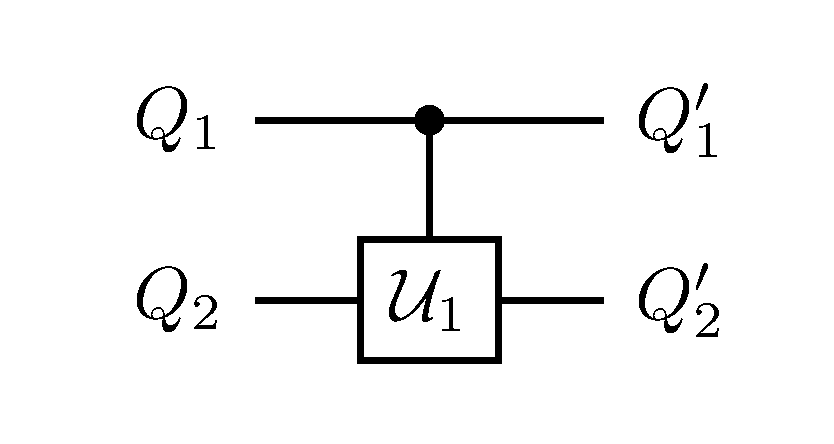
\includegraphics[width=0.8\textwidth]{Immagini/ContrU.pdf}
\end{minipage}
\hspace{-1cm}
\begin{minipage}{0.45\textwidth}
    \begin{equation}
        \text{C}\mathcal{U} = \begin{pmatrix}
            \mathbb{1} & \mathbb{0}\\
            \mathbb{0} & \mathcal{U}
        \end{pmatrix}.
    \end{equation}
\end{minipage}

\noindent
Where, in the graphical representation the dot describe the control qubit.

\paragraph{Swap.} This gate is in reality a simple circuits constructed using three CNOT gates in order, and the reason of the name can be easily seen by the truth table.

\begin{minipage}{0.45\textwidth}
    \centering
    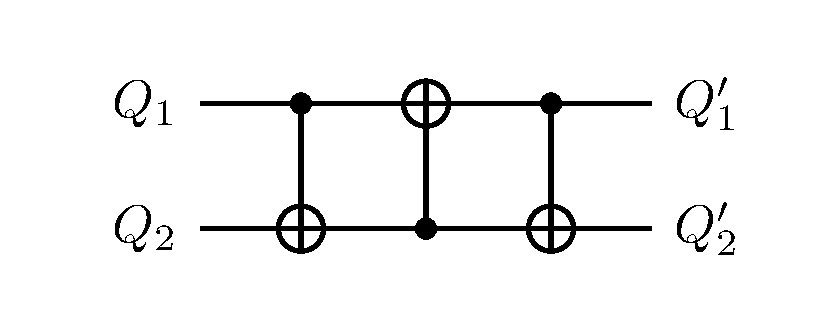
\includegraphics[width=0.9\textwidth]{Immagini/SwapCirc.pdf}
\end{minipage}
\hspace{-1cm}
\begin{minipage}{0.45\textwidth}
    \centering
    \begin{tabular}{c|c}
        \textbf{IN} & \textbf{OUT}\\
        \midrule
        $\ket{00}$ & $\ket{00}$\\
        $\ket{01}$ & $\ket{10}$\\
        $\ket{10}$ & $\ket{01}$\\
        $\ket{11}$ & $\ket{11}$
    \end{tabular}
\end{minipage}
\vspace{0.3cm}

\noindent
Thus, one can see that the effect is literally the one of swapping the states of the qubit. This is a simple and clever operation that can be written in a simple matrix form thanks to the fact that we know the matrix describing the gate of the circuit of which is formed. Therefore, we can write down the final gate by simply matrix multiplying the gates of which is composed in the right order and then having the following one described by its own simbol

\begin{minipage}{0.45\textwidth}
    \centering
    \includegraphics[width=0.8\textwidth]{Immagini/Swapsim.pdf}
\end{minipage}
\hspace{-1cm}
\begin{minipage}{0.45\textwidth}
    \begin{equation}
        \text{SWAP} = \begin{pmatrix}
            1 & 0 & 0 & 0 \\
            0 & 0 & 1 & 0 \\
            0 & 1 & 0 & 0 \\
            0 & 0 & 0 & 1 \\
        \end{pmatrix}.
    \end{equation}
\end{minipage}

\paragraph{Bell.} This is a simple circuit that nevertheless is really important since allow for the creation of particular states of major interest in physics, the Bell's states. The latter are four quantum mechanical states defined as follows
\begin{align}
    &\psi^{\pm} = \frac{1}{\sqrt{2}}\left( \ket{00} \pm \ket{11} \right), &\phi^{\pm} = \frac{1}{\sqrt{2}}\left( \ket{01} \pm \ket{10} \right).
\end{align}
They are mostly important in the theoretical study of spin states, but they appear also in other areas of QM. Thus, we want to describe a circuit that is able to prepare the system in those states and the way in which this can be done is the following

\begin{minipage}{0.45\textwidth}
    \centering
    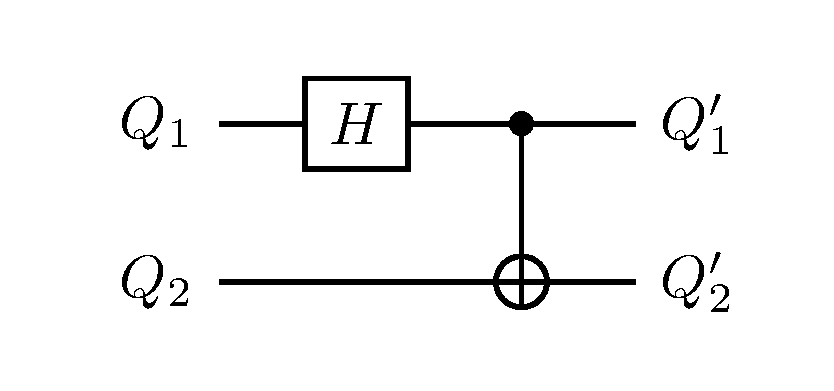
\includegraphics[width=\textwidth]{Immagini/BellCirc.pdf}
\end{minipage}
\hspace{-1cm}
\begin{minipage}{0.45\textwidth}
    \centering
    \begin{tabular}{c|c}
        \textbf{IN} & \textbf{OUT}\\
        \midrule
        $\ket{00}$ & $\psi^+$\\
        $\ket{01}$ & $\phi^+$\\
        $\ket{10}$ & $\psi^-$\\
        $\ket{11}$ & $\phi^-$
    \end{tabular}
\end{minipage}
\vspace{0.3cm}

\noindent
Basically, based on the initial state of the system we are able to generate one of the four Bell state and then study their behavior in specific circuits. 

\ex{Circuit solving}
{
    As a scrupulous, I want to see the computation of the Bell's gate output for the case $\ket{10}$ just to show the reader how effectively solve the circuit. At first the Hadamart gate is used on the first qubit
    \begin{equation}
        H\ket{1}\ket{0} = \frac{1}{\sqrt[]{2}}\left( \ket{0}\ket{0} - \ket{1}\ket{0} \right) = \frac{1}{\sqrt[]{2}}\left( \ket{00} - \ket{10} \right),
    \end{equation}
    then the CNOT operation is applied using the first qubit as control, having the final result
    \begin{equation}
        \psi^+ = \frac{1}{\sqrt{2}} = \left( \ket{00} - \ket{11} \right)
    \end{equation}
}

\subsection{N qubits gates}

We can now step into assuming to have a general number of qubits to work with and see how some general gates can effectively be created also in this case, in particular two main types of gates play a huge role in the whole theory of quantum computers.

\paragraph{Toffoli.} This is a specific 3-qubit gate that has the aim of making a control NOT gate using two different controls. Basically, having two controls the idea is to apply the NOT to the target if and only if both the two controls are in state $\ket{1}$. For this reason the gate is also called CCNOT and has the following matrix and circuit representation

\begin{minipage}{0.45\textwidth}
    \centering
    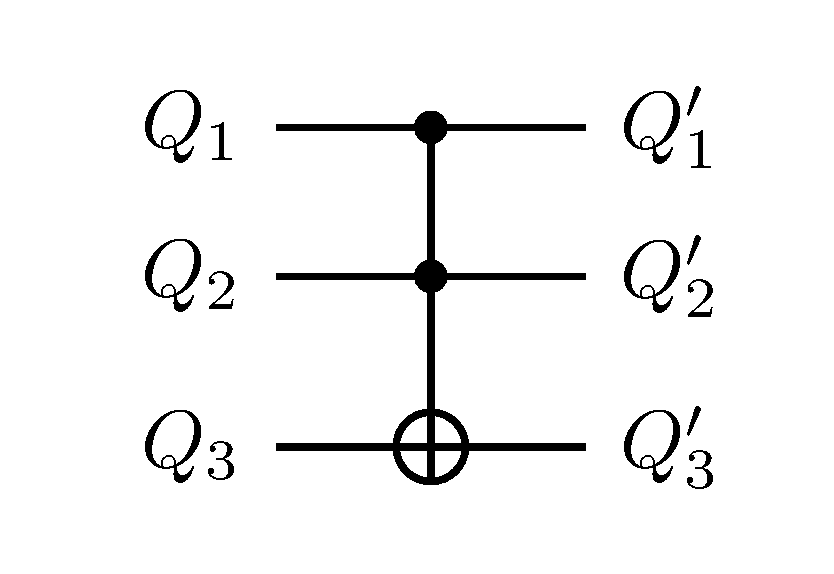
\includegraphics[width=\textwidth]{Immagini/Toffoli.pdf}
\end{minipage}
\begin{minipage}{0.45\textwidth}
    \begin{displaymath}
        \text{CCNOT} = \begin{pmatrix}
            1 & 0 & 0 & 0 & 0 & 0 & 0 & 0\\
            0 & 1 & 0 & 0 & 0 & 0 & 0 & 0\\
            0 & 0 & 1 & 0 & 0 & 0 & 0 & 0\\
            0 & 0 & 0 & 1 & 0 & 0 & 0 & 0\\
            0 & 0 & 0 & 0 & 1 & 0 & 0 & 0\\
            0 & 0 & 0 & 0 & 0 & 1 & 0 & 0\\
            0 & 0 & 0 & 0 & 0 & 0 & 0 & 1\\
            0 & 0 & 0 & 0 & 0 & 0 & 1 & 0\\
        \end{pmatrix}
    \end{displaymath}
\end{minipage}

\noindent
The task of writing down the truth table from the matrix representation is left to the reader to effectively see how the aim of applying a NOT to the last qubit only if the first two are in $\ket{1}$ is accomplished.

\paragraph{N control.} These gates are a generalization of the Toffoli one to an N number of control and an M number of targets. In general the idea is to apply a general M-qubit gate $\mathcal{U}$ to the targets qubits if the N controls are in the state $\ket{1}$, the general form of the matrix is analogous to the one already seen for the CU gates and the circuit is also totally analogous to the Toffoli and CU one. 
    \section{Performing classical computations}

The quantum computer seems to have all the potential of performing computations that normal computers can't do, but it's not obvious that they can still perform the task of a normal one. That is a problem, in fact creating computers that are not able to perform simple tasks would be useless for us, and so we want to demonstrate that this isn't the case. 

The question "can quantum computers do classical computations?" comes from the doubt that in the possible operations that can be done on the qubits may not be able to simulate the two general operations that give rise to all the classical logic. These operations are the NAND gate and the COPY one, which together forms the building block of all the other possible operations. The first one is the \textbf{universal operation} of classical logic meaning that every circuit can be constructed using only NAND opeartions, while the latter constitute a problem due to some properties of QM that makes coping a non-trivial matter. Here we want to take the two properties one at a time and demonstrate that QC can perform both using the \textbf{Toffoli gate}.

\subsection{NAND operation}

The possibility of a QC to perform the NAND operation is not obvious, and the reason for that is the fact that all the quantum operations that we can perform on a qubit are invertible which the NAND is not. Basically it's not sure that a non-invertible operation can be constructed using invertible ones, or better if we can represent it using an invertible operation on a qubit. Fortunately turns out that performing the NAND on qubit is not only possible, but simple. The idea is using a Toffoli gate and setting one of the three qubits to $\ket{1}$, obtaining as output the NAND of the other two as we can see in the following circuit.

\begin{minipage}{0.4\textwidth}
    \centering
    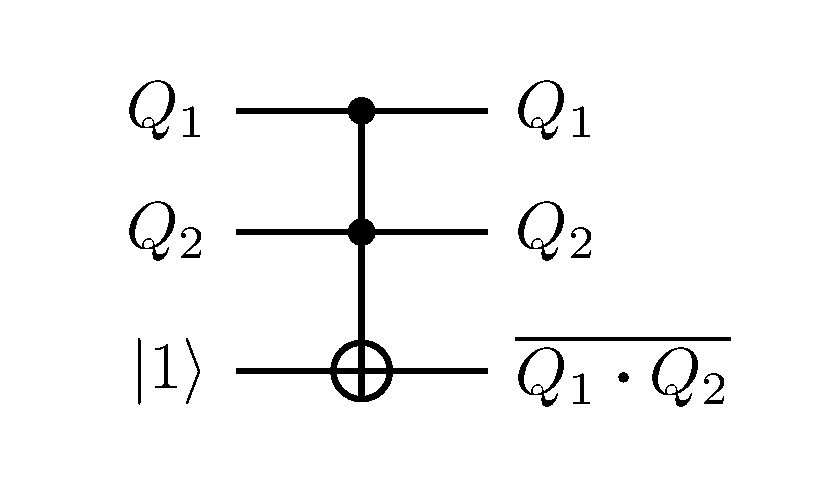
\includegraphics[width=\textwidth]{Immagini/NAND.pdf}
\end{minipage}
\begin{minipage}{0.45\textwidth}
    \centering
    \begin{tabular}{c|c}
        \textbf{IN} & \textbf{OUT}\\
        \midrule
        $\ket{001}$ & $\ket{001}$\\
        $\ket{011}$ & $\ket{011}$\\
        $\ket{101}$ & $\ket{101}$\\
        $\ket{111}$ & $\ket{110}$
    \end{tabular}
\end{minipage}

\noindent
Which clearly reconstruct the NAND as wanted, meaning that using QC we are able to recreate every possible classical circuit.

\subsection{Coping information}

First, we shall clarify why this operation represent a problem inside quantum circuits, and the reason is intrinsic inside QM and in the known result called \textbf{non-cloning theorem}, which states the following.
\thm{Non-cloning}
{
    \label{thm:cloning}
    Taken a state $\ket{\psi}$ of a system of qubit, it does not exist a unitary operation $\mathcal{U}$ with the following property
    \begin{equation}
        \label{eq:noCloning}
        \mathcal{U}\left( \ket{\psi}\otimes \ket{s} \right) = \ket{\psi}\otimes \ket{\psi},
    \end{equation}
    where $\ket{s}$ is another arbitrary state.
}
\pf{Proof}
{
    Let's imagine that such operation exist, and take three arbitrary states $\ket{\psi}$, $\ket{\phi}$ and $\ket{s}$. Since $\mathcal{U}$ is unitary the following relation must hold true
    \begin{equation}
        \braket{s\phi}{\psi s} = \braket{s}\braket{\phi}{\psi} = \mel{s\phi}{\mathcal{U}^\dagger \mathcal{U}}{\psi s},
    \end{equation}
    but using relation \eqref{eq:noCloning} and the normalization of the states it's possible to see that the latter equation becomes
    \begin{equation}
        \braket{\phi}{\psi} = \braket{\phi}{\psi}^2.
    \end{equation}
    This is not true in general, but only if we select carefully the two states in order for them to respect this relation. Otherwise, the operation $\mathcal{U}$ cannot be unitary and therefore is not a viable quantum gate.
}

This result may seem a problem by all means, but already in the proof is hidden the answer to overcome it. In fact, we have said that a cloning operation can exist if the starting states are selected carefully so that the norm of the states is conserved. In practice this means that we can use a Toffoli gate with two entries selected in a specific way to obtain the following copy gate.

\begin{minipage}{0.4\textwidth}
    \centering
    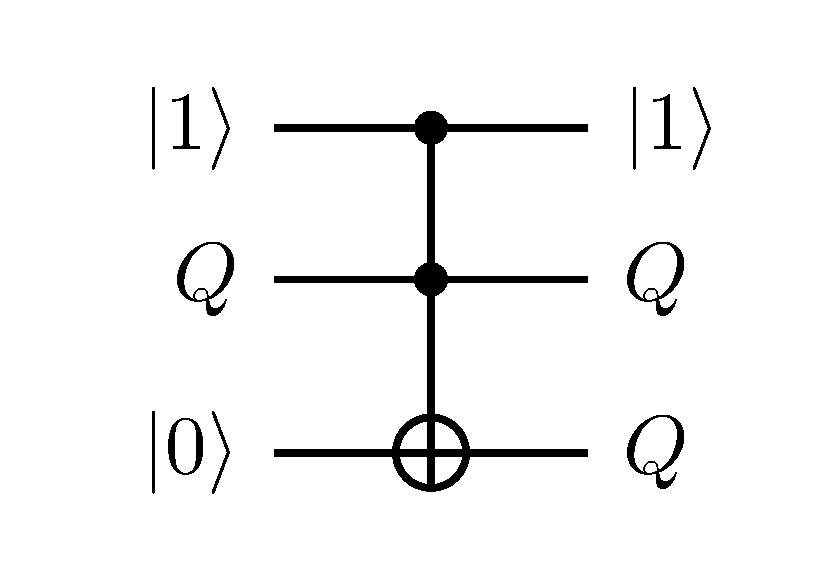
\includegraphics[width=\textwidth]{Immagini/Copy.pdf}
\end{minipage}
% \hspace{-1cm}
\begin{minipage}{0.45\textwidth}
    \centering
    \begin{tabular}{c|c}
        \textbf{IN} & \textbf{OUT}\\
        \midrule
        $\ket{100}$ & $\ket{000}$\\
        $\ket{110}$ & $\ket{111}$
    \end{tabular}
\end{minipage}

\noindent
In this way also coping information to one qubit to another can be done always using the Toffoli gate, making it probably the most important of all, and demonstrating that QC can perform all classical computations along with the unexplored quantum ones.
    \section{Measurements}

During the first section we have introduced the concept of measure as a set $\{ \hat{\Pi}_n \}_{n\in\mathcal{I}}$ of operators that allow us to evaluate the probability of having a certain outcome $\lambda_n$ for the measure of a physical quantity $\Lambda$. Nevertheless, even if we have listed the main properties that such operators should have we didn't specify the forms that they can possess. It is now time to introduce the main way in which such set of operators can present themselves and how they will work inside quantum circuits.

\subsection{Projection valued measurement}

If we take a look back to the different properties stated in Def. (\ref{def:measure}) an idea should arise, especially by looking at the collapse condition. The latter, in fact, can be thought as the state of the system gets projected into a certain state that posses a definite value of the physical quantity we are interested in measuring. In fact, it's easy to see how the following is true
\begin{align}
    &\hat{\Pi}_n \ket{\psi_n} = \ket{\psi_n}, &p_n = \ev{\hat{\Pi}_n^\dagger\hat{\Pi}_n}{\psi_n} = 1.
\end{align}
Operators that posses this effect of taking a general state $\ket{\psi}$ and taking it into another are really known in mathematics and are called \textbf{projector operators}, represented as $\hat{P}$. This type of operator is defined, in particular, by two main conditions
\begin{align}
    \label{eq:ProjDef}
    &\hat{P}^\dagger = \hat{P}, & \hat{P}^2 = \hat{P},
\end{align}
these two properties are enough to give $\hat{P}$ a lot of power allowing it to define alone a subspace of the vector space in which is working. In our case this means
\begin{equation}
    \mathcal{P} = \left\{ \left.\ket{\psi}\right| \exists \ket{\phi} \in \mathcal{H}: \ket{\psi} = \hat{P}\ket{\phi} \right\},
\end{equation}
basically we are aiming to create a set $\{ \hat{P}_n \}$ so that $\mathcal{P}_n$ is the eigenspace of $\lambda_n$. Therefore, it's easy to understand that on a general ground we are searching for a specific type of measure constructed using projectors, that will take the following specific name and definition.
\dfn{Projection valued measurement}
{
    We will call projection valued measurement, or PVM, a set of operators $\{ \hat{P}_n \}_{n\in\mathcal{I}}$ so that $\hat{P}_n$ is a projector and the whole set is a measure.
}

To find out the right projectors to create the complete set we can simply use the properties of the observable in QM. An observable quantity is represented in QM using an operator $\hat{\Lambda}$ and the possible values that $\Lambda$ can take, the outcomes, are the eigenvalues of that operator $\lambda_n$. Nevertheless, for a general operator $\lambda_n$ can be complex, or worst they can not exist, that is a problem since is absurd to mesure a complex number in an experiment, therefore we will make a further assumption giving out the following definition.
\dfn{Observables}
{
    An observable $\Lambda$ in QM is represented by a hermitian operator $\hat{\Lambda}$, so that
    \begin{equation}
        \hat{\Lambda}^\dagger = \hat{\Lambda}.
    \end{equation}
}
\noindent
A really important theorem of linear algebra called \textbf{spectral theorem} allow us to say that, with this further assumption of hermiticy, the operator can be diagonalyzed and the eigenvalues are all real. Along with that, the spectral theorem also allow us to say that a set of eigenstates $\{\ket{\psi_n}\}$ with the following properties exist
\begin{equation}
    \label{eq:BaseDef}
    \hat{\Lambda}\ket{\psi_n} = \lambda_n\ket{\psi_n}, \hspace{2cm} \braket{\psi_n}{\psi_m} = \delta_{nm}, \hspace{2cm} \sum_n \ketbra{\psi_n}{\psi_n} = \mathbb{1},
\end{equation}
forming an orthonormal base for $\mathcal{H}$. These properties should hint us that the set of projectors that we want to create to measure $\Lambda$ may be the ones that project onto the eigenspace generated by $\ket{\psi_n}$, and we can easily see how that is the case. 

\thm{Observable PVM}
{
    Taken $\hat{\Lambda}$ an observable the set of projectors $\{ \hat{P}_n \}_{n\in\mathcal{I}}$ onto the orthonormal base of eigenstate $\{\ket{\psi_n}\}_{n\in\mathcal{I}}$ of $\hat{\Lambda}$ forms a measure for the observable itself called \textbf{Projection valued measurement}.
}
\pf{Proof}
{
    We are going to define the projector $\hat{P}_n$ as follows
    \begin{equation}
        \hat{P}_n = \ketbra{\psi_n},
    \end{equation}
    which can be easily seen it's a projector, the demonstration is left to the reader. We want to see how all the requirement in Def. (\ref{def:measure}) are verified, we can start from the probability by taking a general state $\ket{\psi}$ and writing
    \begin{align}
        &\ket{\psi} = \sum_n c_n\ket{\psi_n},   & p_n = \ev{\hat{P}^\dagger_n\hat{P}_n}{\psi} = \ev{\hat{P}_n}{\psi} = \abs{c_n}^2.
    \end{align}
    Where I have first written the expansion of $\ket{\psi}$ on the orthonormal base and then used the properties in \eqref{eq:ProjDef} and \eqref{eq:BaseDef} to obtain the probability. It's possible to see how the values of $\abs{c_n}^2$ effectively represents probabilities since also the condition \eqref{eq:MeasureCompleteCondition} is respected by the set of operators defined thanks to the completeness condition of the orthonormal base
    \begin{equation}
        \sum_n \hat{P}^\dagger_n\hat{P}_n = \sum_n \hat{P}_n = \sum_n \ketbra{\psi_n} = \mathbb{1}.
    \end{equation}
    Therefore, the first condition for having a measure is respected. We can now see how also the second one is obtained as we want since we can write
    \begin{equation}
        \ket{\psi_n} = \frac{\hat{P}\ket{\psi}}{\sqrt{\ev{\hat{P}^\dagger_n\hat{P}_n}{\psi}}} = \frac{c_n}{\sqrt{\abs{c_n}^2}}\ket{\psi_n} = e^{i\theta}\ket{\psi_n},
    \end{equation}
    and since a complex phase doesn't change the physical state of the system the wanted result is achieved.
}

\ex{Qubit PVM}
{
    To make an example we can use a qubit, where we can imagine measuring the state as $\ket{1}$ or $\ket{0}$, so a computational base measurament. We can also easily imagine what is the form of the operator, the observable, that has them as eigenstates
    \begin{align}
        &Z = \begin{pmatrix}
            1 & 0\\
            0 & -1
        \end{pmatrix}, &Z\ket{i} = \lambda_i\ket{i},
    \end{align}
    where it's easy to see, by using the $\mathbb{C}^2$ representation of the states, how $\lambda_0 = 1$ and $\lambda_1 = -1$. This means that for every state $\ket{\psi}$ we can measure the probability of a certain outcome, state $\ket{1}$ or $\ket{0}$, to appear by using the set of operators defined by $\hat{P}_i = \ketbra{i}$ given as matrix by
    \begin{align}
        &P_0 = \begin{pmatrix}
            1 & 0\\
            0 & 0
        \end{pmatrix},
        &P_1 = \begin{pmatrix}
            0 & 0\\
            0 & 1
        \end{pmatrix}.
    \end{align}
    Applied to a general vector they will give in general the first or second component, respectively.
}

\subsection{Positive operator valued measurement}

In the PVM description of measure that we have given just now we use projector operators to predict the probabilities, which posses a series of properties that makes them really well suited for the task. Nevertheless, they are not the only possible choice, in particular such projectors posses the property of being hermitian that general measures can totally not have. We want so to see a case where another type of measure respect to the PVM can be a better choice to study the system.

Let's imagine having a qubit and a quantum circuit that is able to prepare it in two states given by
\begin{align}
    &\ket{\psi_1} = \ket{0}, & \ket{\psi_2} = \frac{\ket{0} + \ket{1}}{\sqrt{2}}.
\end{align}
We want to see if we are able to understand which state after a measure. Using the PVM measure of a qubit using $Z$ as an observable we can easily see how $\ket{\psi_1}$ posses a probability equal to $1$ of being in state $\ket{0}$, while $\ket{\psi_2}$ has $p_i = 1/2$ for both states. This means that if I take a measure and the outcome is $\lambda = -1$ I know that the only state that can have that outcome is $\ket{\psi_2}$ since has a non-zero probability of being in state $\ket{1}$. Instead, if the result is $\lambda = 1$ I can't say which one of the two state is the right one. We can also understand why we are not able to decide, since the two states that we are working with are not orthogonal respect to the computational base and so $\ket{\psi_2}$ has non-zero probability of being in both states. Therefore, we would like to use a set of operators that instead are able to give us this property, and a possible way of obtaining them is by taking $\{ \hat{\Pi}_n \}$ so that
\begin{equation}
    \hat{\Pi}_n^\dagger\hat{\Pi}_n = \hat{E}_n,
\end{equation}
are \textbf{positive valued operators}. In this way we are allowed to define as our operators the following objects
\begin{align}
    &\hat{E}_1 = \ketbra{1}, &\hat{E}_2 = \left( \frac{\ket{0} - \ket{1}}{\sqrt{2}} \right)\left( \frac{\bra{0} - \bra{1}}{\sqrt{2}} \right),
\end{align}
basically the projector on the states that are orthogonal to the ones that we were looking at. Nevertheless, the set composed by $\hat{E_1}$ and $\hat{E}_2$ is not sad to respect the relation \eqref{eq:MeasureCompleteCondition} meaning that we are needed to add a third element in general that allow for the set to be a measure
\begin{equation}
    \hat{E}_3 = \mathbb{1} - \hat{E}_2 - \hat{E}_1.
\end{equation}
Then, using this new set we are able to obtain a more satisfying result since the now the possible outcomes of the measurement are three. In fact, we can imagine that doing a measure using $\{\hat{E}_n\}$ is experimentally equivalent to obtain three possible outcomes $\lambda_n$ where the probabilities of the outcomes for the two states respectively are
\begin{align}
    &\ev{\hat{E}_i}{\psi_1} = \begin{cases}
        p_1 = 0\\
        p_2 \neq 0\\
        p_3 \neq 0
    \end{cases},
    &\ev{\hat{E}_i}{\psi_2} = \begin{cases}
        p_1 \neq 0\\
        p_2 = 0\\
        p_3 \neq 0
    \end{cases}.
\end{align}
Therefore, now after a measure we are able to say that if the outcome is $\lambda_1$ or $\lambda_2$ the result is state $\ket{\psi_1}$ or $\ket{\psi_2}$ respectively, while $\lambda_3$ is telling us that the measure is not satisfying since we can't distinguish the two states. This may seem not so different respect to the PVM measure since still we have the case where the single measure can distinguish the two cases, but here we have also an outcome that tells us with certainty to have $\ket{\psi_2}$ that we didn't have before. Also, it is possible to demonstrate that the probability of an not satisfying measure is minimized by this set.

Therefore, with this simple case we have seen how the definition of measure in reality leaves large freedom in the choice of the operator set and not only projectors. In fact, we can now generaly define also the positive operator valued measurement as follows.
\dfn{POVM}
{
    We will call positive operator valued measurement a set of operators $\{ \hat{E}_n \}_{n\in\mathcal{I}}$ so that $\hat{E}_n$ is a positive valued operator and the whole set represent a measure.
}
\noindent
This definition is much more general than PVM and can allow for better result in terms of computations as we have seen in the example shown beforehand. Nevertheless, the problem of these measures is that we actually don't know how to represent them in practice. In fact, for PVM the definition was made starting from a physical observable while here the physical representation is much more hidden. Still, doesn't mean that don't exist. Is possible to demonstrate that whatever measure, can be represented into a higher dimensional space through a unitary transformation composed a PVM, in this way everything can be physically interpreted. We can so state the following result in terms related to quantum computers applications as follows.
\thm{Representation of measures}
{
    Any generalized measure on a system of $N$ qubit $\mathcal{H}_Q$ can be realized as a PVM with the aid of auxiliary qubit and a unitary operator.
}
\pf{Proof}
{
    Imagine having a general measure $\{ \hat{\Pi}_n \}_{n\in\mathcal{I}}$ acting on $\mathcal{H}_Q$, we can take an orthonormal set $\{ \ket{m} \}_{m\in\mathcal{I}'}$, with $\#\mathcal{I} = \#\mathcal{I}'$, of states $\ket{m}\in \mathcal{H}_Q$ and construct an auxiliary space as
    \begin{align}
        &\mathcal{H}_{tot} = \mathcal{H}_Q\otimes \mathcal{H}_M, &\mathcal{H}_M = \text{span}\{\ket{m}\}.
    \end{align}
    So, a general state inside the auxiliary space can be written as $\ket{\psi}\ket{s}$, with $\ket{\psi}\in \mathcal{H}_Q$ and $\ket{s}\in\mathcal{H}_M$. Now, we define the transformation $\mathcal{U}$ as follows
    \begin{equation}
        \mathcal{U}\ket{\psi}\ket{s} = \sum_n \left( \hat{\Pi}_n\ket{\psi} \right)\ket{m},
    \end{equation}
    which can be seen to be a unitary operator since the following relation can be obtained
    \begin{equation}
        \bra{s}\bra{\psi}\mathcal{U}^\dagger\mathcal{U}\ket{\phi}\ket{s} = \sum_{mm'}\mel{\psi}{\hat{\Pi}_{m'}^\dagger\hat{\Pi}_m}{\phi}\braket{m'}{m} = \sum_m \mel{\psi}{\hat{\Pi}_{m}^\dagger\hat{\Pi}_m}{\phi} = \braket{\psi}{\phi}.
    \end{equation}
    Where the relation $\braket{m}{m'} = \delta_{mm'}$ and $\sum_n \hat{\Pi}_{m'}^\dagger\hat{\Pi}_m = \mathbb{1}$ have been used during the process, demonstrating that $\mathcal{U}$ conserve the norm of the space being so unitary. Next we can define the projection operators to be given by the following
    \begin{equation}
        \hat{P}_m = \mathbb{1}_Q \otimes \ketbra{m},
    \end{equation}
    creating a PVM set of measure. Then, we can see how the operator $\hat{P}_m\mathcal{U}$ act on a general state of the whole space as
    \begin{equation}
        \hat{P}_m\mathcal{U}\ket{\psi}\ket{s} = \sum_{m'} \left( \hat{\Pi}_n\ket{\psi} \right)\braket{m}{m'} \ket{m}= \hat{\Pi}_m\ket{\psi}\ket{m}.
    \end{equation}
    This is a powerful result since we can already see how this set of operations is able to reproduce the general measure in all of it's fascion. We can start by seeing how the probabilities that predicts are the same
    \begin{equation}
        p_m = \bra{s}\bra{\psi}\mathcal{U}^\dagger\hat{P}_m^\dagger\hat{P}_m\mathcal{U}\ket{\psi}\ket{s} = \ev{\hat{\Pi}_n^\dagger\hat{\Pi}_n}{\psi}.
    \end{equation}
    Thus, also the projection remains unchanged under the effect of this operator since
    \begin{equation}
        \frac{\hat{P}_m\mathcal{U}\ket{\psi}\ket{s}}{\sqrt{\bra{s}\bra{\psi}\mathcal{U}^\dagger\hat{P}_m^\dagger\hat{P}_m\mathcal{U}\ket{\psi}\ket{s}}} = \frac{\hat{\Pi}_m\ket{\psi}}{\sqrt{\ev{\hat{\Pi}_n^\dagger\hat{\Pi}_n}{\psi}}}\ket{m} = \ket{\psi_m}\ket{m}.
    \end{equation}
    Therefore, all the properties of the general measure are conserved, meaning that $\{ \hat{P}_m\mathcal{U} \}$ successfully represent it.
}
\noindent
This result is telling is that doesn't matter with measure we are using we can always add a number of qubit so that the space becomes larger by a $\mathcal{H}_M$ with dimensions equal to the number of outcomes you want to measure and use a normal PVM along with a unitary transformation defined by the measure itself. In this way we can always use the same $Z$ gate seen in the PVM example to measure the auxiliary qubit and based on the value of their state, which gives $\ket{m}$, we can know the outcomes of the others, since $\ket{m}$ correspond to a collapsed $\ket{\psi_m}$ and so $\lambda_m$ as outcome.

\nt
{
    This whole theory was though first by Von Neumann which tried to create it to describe the collapse on the wavefunction in a rigorous way. In particular He though that an experimental apparatus in general was the auxiliary system $\mathcal{H}_M$ that taking the measure made the system collapse in the way we have seen.
}

\subsection{Measurements and circuits}

Measuring is an important feature inside a quantum circuits since at the end of the manipulations we also need to know the result of the operations contained in the qubits states. In general, we are going to see how the measurement works inside a quantum circuit and their properties. First, we shall keep in mind that usually all the quantum computers are able to perform measurements mainly in the computational basis, meaning of the observable $Z$. This is due to a matter of experimental convenience, but lead us to try to reconduce every possible measure to that one.

% TODO: Qua devi fare l'esempio di come si misura uno stato anche se è descritto in termini di un'altra base facendo le rotazioni, qui ci può stare un disegno in modo tare da introdurre la notazione che non sarebbe affatto male, anche per la notazione del bit classico.

% TODO: Devi metterci il principio del "lo puoi mettere dove cazzo ti pare" e del "misura implicita"

% TODO: Controllo classico o controllo quantistico, ma lo puoi infilare anche dentro al principio del, lo puoi mettere dove cazzo ti pare("anzi, fai l'esempio con quello così te lo levi subito")
    \section{Entanglement}

The concept of entanglement comes from the need of describing the difference of certain type of states respect to others. In particular, we can understand it by first defining a really simple type of state called separable that has the following form.
\dfn{Separable state}
{
    Taken a state $\ket{\psi}\in\mathcal{H}_1\otimes\mathcal{H}_2$ it's called separable if $\exists \ket{\phi_1}\in \mathcal{H}_1, \ket{\phi_2} \in \mathcal{H}_2$ so that we can write
    \begin{equation}
        \ket{\psi} = \ket{\phi_1}\otimes\ket{\phi_2}.
    \end{equation}
}
\noindent
This type of states are really simple since we can decompose them into simpler once and work with them. To make an example we can see how the state $(\ket{01} + \ket{00})/\sqrt{2}$ is a separable one since
\begin{equation}
    \frac{\ket{01} + \ket{00}}{\sqrt{2}} = \ket{0}\left( \frac{\ket{0} + \ket{1}}{\sqrt{2}} \right),
\end{equation}
holds true and so can be decomposed. Nevertheless, we shall not go much further to find out more complex states that cannot be decomposed for which we need to work in the higher dimensional space like the Bell's state $(\ket{01} + \ket{10})/\sqrt{2}$. Those are entangled states, whose definition is therefore really simple as.
\dfn{Entangled states}
{
    \label{def:Entangl}
    A state $\ket{\psi}\in\mathcal{H}_1\otimes\mathcal{H}_2$ it's called entangled if it's not separable.
}
\noindent
Therefore, the mathematical definition of entanglement seems really simple, but the physical consequences are not, and we shall see together why this is one of the main powers of QC.

\ex{}
{
    To make an example of how powerful the entanglement can be we can see how in theory we can transport the information of two bits, so $00$, $01$, $10$ or $11$, transmitting only one qubit. The idea is that two people, Alice and Bob, posses two qubit that are entangled in the following Bell state
    \begin{equation}
        \ket{\psi^+} = \frac{\ket{00} + \ket{11}}{\sqrt{2}},
    \end{equation}
    then Alice can perform one of four operations on it's qubit based on what wants to transmit to Bob. In particular the following choices can be made
    \begin{align*}
        &\text{Operation}               &\text{Final state}\\
        &\ket{00} \to \mathbb{1}        &\ket{\psi^+}\hspace{0.4cm}\\
        &\ket{01} \to Z                 &\ket{\psi^-}\hspace{0.4cm}\\
        &\ket{10} \to X                 &\ket{\phi^+}\hspace{0.4cm}\\
        &\ket{11} \to iY                &\ket{\phi^-}\hspace{0.4cm}
    \end{align*}
    So, based on the information that we want to send we have performed an operation of the Alice qubit to obtain a different Bell state. Then, Alice only need to send the qubit to Bob which need to perform a two qubit measure using the Bell's base and the state that will obtain will correspond to the selected two bit information obtained with the transport of only one qubit.
}

\nt
{
    This definition of Entanglement is not really the most general one that can be used. In fact, the Def. (\ref{def:Entangl}) it's a specific one called bi-entanglement since only two Hilbert spaces are counted, but the most general called n-entanglement count for $\ket{\psi}\in \bigotimes_{i=1}^n \mathcal{H}_i$. Nevertheless, for QC application only the bi-entanglement plays an important role.
}

\subsection{Quantum teleportation}

The first real important application of entanglement that we will see it's the quantum protocol for the quantum teleportation of information. Basically we want to teleport a quantum state from one qubit to another, so that no matter is transported to one place to another but only the state of the qubits is changed transporting information. Also, at first site one can also think that the cloning theorem would be violated in a situation of this type, but that is not the case, and we will see why.
\begin{figure}[b]
    \centering
    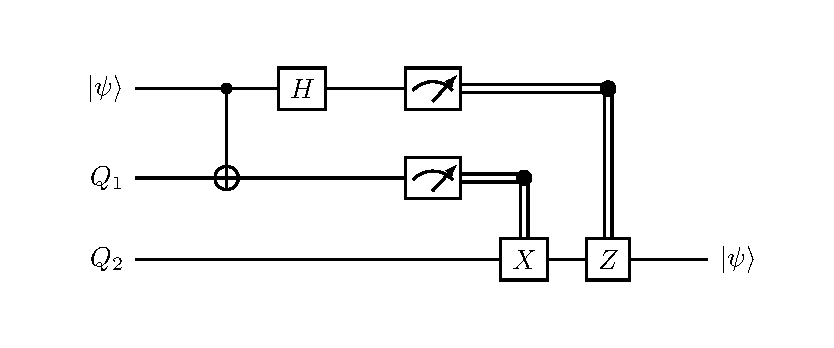
\includegraphics[width=0.8\textwidth]{Immagini/QuanTeleport.pdf}
    \caption
    {
        Quantum teleportation circuit for a quantum computer, see how it involves the measuring of two qubit to control two operations.
    }
    \label{fig:QuanTeleport}
\end{figure}

The circuit that is used in order to perform the teleportation protocol is reported in \figref{fig:QuanTeleport}, and consist in the use of two qubit in order to transport a general state $\ket{\psi} = a\ket{0} + b\ket{1}$ into one of those qubit. Thus, we want to understand how this is possible in general, and to do that let's pretend that the two qubit $\ket{\psi}$ and $Q_1$ are in possession of Alice, while $Q_2$ is with Bob. We will need that the two qubit $Q_1$, $Q_2$ are entangled in a $\ket{\psi^+}$ Bell state, then we can place them at whatever distance, so that Alice and Bob can be also on different planets. In this situation Alice will perform a series of operation on her qubit starting with a CNOT, to understand what this operation will do on the system we need first to look at the state of the hole three qubit, which will be
\begin{equation}
    \ket{\psi Q_1Q_2} = \left( a\ket{0} + b\ket{1} \right)\left( \frac{\ket{00} + \ket{11}}{\sqrt{2}} \right) = \frac{1}{\sqrt{2}}\left[ a\ket{000} + a\ket{011} + b\ket{100} + b\ket{111} \right].
\end{equation}
Then we can easily perform the CNOT on the first two qubit ending up in the following state
\begin{equation}
    \frac{1}{\sqrt{2}}\left[ a\ket{000} + a\ket{011} + b\ket{110} + b\ket{101} \right],
\end{equation}
on which the Hadamart tranformation is applied on the first qubit, which we shall remember that transforms $\ket{0}$ in $\ket{+}$ and $\ket{1}$ in $\ket{-}$. Therefore, we will have the following form
\begin{equation}
    \frac{1}{2}\left[ a\ket{000} + a\ket{100} + a\ket{011} + a\ket{111} + b\ket{010} - b\ket{110} + b\ket{001} - b\ket{101} \right],
\end{equation}
which can be rewritten by seeing how inside it four separable states can be found out, having
\begin{equation}
    \frac{1}{2}\left[ \ket{00}\left( a\ket{0} + b\ket{1} \right) + \ket{01}\left( a\ket{1} + b\ket{0} \right) + \ket{10}\left( a\ket{0} - b\ket{1} \right) + \ket{11}\left( a\ket{1} - b\ket{0} \right) \right].
\end{equation}
At first sight this state may seem nothing special, but if the states inside parentheses are inspected one could find out different forms of $\ket{\psi}$ obtaining
\begin{equation}
    \frac{1}{2}\left[ \ket{00}\left( \ket{\psi} \right) + \ket{01}\left( X\ket{\psi} \right) + \ket{10}\left( Z\ket{\psi} \right) + \ket{11}\left( XZ\ket{\psi} \right) \right].
\end{equation}
We have so created a state where the two qubit state given by Alice's couple is entangled to the qubit of Bob, which will poses the $\ket{\psi}$ state up to two transformation based on the Alice's values. Therefore, if Alice measure it's two qubit and refers the outcomes to Bob, he can perform the right operations to obtain at the end the final state $\ket{\psi}$ on his qubit. An operation that inside the circuit is described by the two classical controls and can be seen gives the right result keeping in mind that $X^2 = Z^2 = \mathbb{1}$.

Thus, using this protocol a general state $\ket{\psi}$ can be transferred into another qubit at whatever distance without limitations. In fact, the circuit has been performed in several occasions starting from a teleportation distance of some centimeters to the experiment of Anton Zellinger that performed it at nearly one kilometer of distance inside Vienna. Today we are able to transfer states from hearth to satellite, but still this phenomenon result in being quite strange at first sight. Perhaps, as was told earlier, one can say that this \textbf{phenomenon contradicts Thm. (\ref{thm:cloning})} with the coping of a general state into another one. This is a wrong affirmation, since the non-cloning theorem tells that the following operation doesn't exist
\begin{equation}
    \mathcal{U}(\ket{\psi}\otimes\ket{s}) = \ket{\psi}\otimes\ket{\psi},
\end{equation}
while here the starting states have been measured by Alice, meaning that they have collapsed having a result more similar to
\begin{equation}
    \mathcal{U}(\ket{\psi}\otimes\ket{Q_1}\otimes\ket{Q_2}) = \ket{00}\otimes\ket{\psi}.
\end{equation}
Where $\ket{00}$ is only one of the four possible final result obtained. Another apparent contradiction that can be found out inside the teleportation protocol is the fact that \textbf{information seem to pass from one qubit to another faster than the speed of light}. That can't obviously be possible, since relativity forbid it, and in fact that is not the case. The two classical controls that are used inside the circuit solve the problem since in order to obtain the copied state inside $Q_2$ I first need Alice to transmit the result of the measurements to Bob and that classical exchange of information take times.

\subsection{EPR paradox and Bell's inequality}

Since in 2022, the year I'm writing these notes, the Nobel Prize in physics was awarded to Alain Specter, John Clauser and Anton Zeilinger for their experiments on entangled photons, a little part of the course was devoted to the description of the theory they allowed to uncover. To understand it we shall understand that in the first half of 1900 the idea of entanglement was difficult to accept. Especially Einstein was really skeptical about it since at first sight looked like a threat to its restricted relativity with information apparently traveling faster than light. Remained in history Einstein's definition of entanglement as "spooky action at a distance", showing how much he hated it. In this context, great work was putted by Einstein and others physicist in order to see if effectively QM was wrong or, better, not entirely right, meaning that we were still missing something to understand it at its fullest.

In 1935 Einstein, Podolsky and Rosen (EPR) delineated a theory trying to show that QM was indeed not complete, starting by defining what it means for a physical theory to be complete. The line of reasoning starts with the definition of the so-called elements of reality.
\dfn{Elements of reality}
{
    A quantity is called element of reality if it has a value that can be predicted before experiment, basically it's already perfectly known already before taking the measure. A property of this type, for logic, must be owned by the system regardless of what you are making so that exist also before taking the measurement with a precise value.
}
\noindent
This definition is purely based on logic, assuming that if I'm able to know the exact outcome of an experiment before taking the measure then the property that I'm measuring needs to have that value defined intrinsically inside it. Then, the next move is to use this definition to define when a theory is complete.
\dfn{Complete theory}
{
    A physical theory is complete if it contains all elements of reality.
}
\noindent
Using these two definitions, the three theoreticians demonstrated that QM is not complete if we assume the notion of locality. Where, locality was also defined by them as follows.
\dfn{Locality}
{
    Measurements are independent if done in position and time that are not causally related.
}
\noindent
With this they were able to create a thought experiment that demonstrated how some elements of reality were missing inside QM. The experiment that E. P. R. proposed is actually old, today the best way to understand this is by looking at the one proposed by David Bohm in 1951 which shows how spin is what is missing.
\thm{Incompleteness of QM}
{
    Spin is an element of reality that is not contained entirely inside quantum mechanics.
}
\pf{Proof}
{
    We can imagine taking a singlet state of spin which is given by the following Bell state
    \begin{equation}
        \ket{\phi^-} = \frac{\ket{\uparrow\downarrow} - \ket{\downarrow\uparrow}}{\sqrt{2}}.
    \end{equation}
    This state is a peculiar one, since it's possible to demonstrate that has the same form in every possible base. Meaning that if I change the base of representation to an orthonormal couple $\{ \ket{e_1}, \ket{e_2} \}$ the state become
    \begin{equation}
        \ket{\phi^-} = \frac{\ket{e_1e_2} - \ket{e_2e_1}}{\sqrt{2}}.
    \end{equation}
    Thus, if one measures the spin of the system in any direction, so using the right base, the same result will be found out meaning that the spin is an element of reality with a defined value. Nevertheless, in QM we know that the spin operators do not commute, meaning that we can't know both components of the spin at the same time. Basically, even if the whole spin vector is an element of reality quantum mechanics only allows for the partial knowledge of it, meaning that QM does not contain all elements of reality.
}
\noindent
This result showed, in the minds of Einstein and collegues, that the QM is not a complete theory needing still work to find out certain \textbf{hidden variables} whose treated statistically will recreate quanutm mechanics but used normaly will give deterministic results. Basically he was searching for the equivalent of classical mechanics starting from statistical mechanics, where now statistical mechanics is quantum mechanics itself.

This discussion was incredibly interesting at the time, but understanding what the hidden variables were remained more of a phylisofic question for a lot of times untill the idea of Bell. In 1964, he pusblished a paper showing how whatever deterministic real local theory using hidden variables is doomed to fail in reproducing the quantum mechanical result using the following reasoning. He focused his studies on a particualar observable defined using four different ones $Q, S, R$ and $T$, where all of them could only have two possible outcomes $\pm 1$. The observable that we are interested in is the following
\begin{equation}
    \mathcal{L} = QS + RS + RT - QT,
\end{equation}
which posses some interesting properties such as it can have only two possible outcomes $\pm 2$. Bell showed that inside a local real deterministic theory the following result must hold.
\thm{Bell's inequality}
{
    Assuming locality and reality of the four observable composing $\mathcal{L}$ we have that the following relation hold
    \begin{equation}
        \left\langle \mathcal{L} \right\rangle \le 2.
    \end{equation}
}
\pf{Proof}
{
    We will assume that the four observables will be evaluated separetedly in four different measurements, having so that every draw forms the outcome $(q, r, s, t)$ with a probability $P(q, r, s, t)$.  We can so see how the following relation is true since we will have
    \begin{equation}
        \left\langle \mathcal{L} \right\rangle = \sum_{qsrt}(qs + rs + rt - qt)P(q, r, s, t) \le 2\sum_{qrst} P(q, r, s, t),
    \end{equation}
    but the sum of the probability of all possible outcomes need to be normalized at $1$ having so that the wanted relation holds.
}

\noindent
This result allowed to set a condition for the existence of the local hidden variables, the only thing remained to do is to show that quantum mechanics do not respect it. We can so take the following example 
\begin{align}
    &Q=Z_1, &S=-\frac{Z_2 + X_2}{\sqrt{2}},\\
    &R=X_1, &T=\frac{Z_2 - X_2}{\sqrt{2}},
\end{align}
and evaluate the average of $\mathcal{L}$ in the singlet state. From locality, we can say that no correlation exist from the outcomes of the different measurements, so that their probability are independent of each other having
\begin{equation}
    P(q, r, s, t) = P(q)P(r)P(s)P(t).
\end{equation}
Meaning that the following is true
\begin{equation}
    \ev{\mathcal{L}}{\phi^-} = \left\langle QR \right\rangle + \left\langle RS \right\rangle + \left\langle RT \right\rangle - \left\langle QT \right\rangle = 2\sqrt{2} > 2.
\end{equation}
Meaning that QM doesn't respect Bell's inequality and so can't be reconstructed using local hidden variables. This line of reasoning was also proven experimentally by Cluaser first, and then also by Specter with a more refined experiment that reproduced accuratelly the $2\sqrt{2}$ result using photons and not spins. Therefore, local hidden variables will not be the answer to find out a deterministic quantum theory.

From that point on quantum information evolved a lot with the creation of quantum optics and entangled photons, in particualar the last part of the Nobel Prize was given to Zellinger sicne was the first to perform quantum teleportation in open air at a far distance in Vienna. He teleported a state using entangled photons from one part to the other of the Danube river.
    \section{Quantum algorithms}

It's now to see some important quantum circuits that can be used in practice in order to obtain interesting results or behaviour inside a quantum computer. A lot of them will be not usefull per se, but are really important for the creation of larger and more powerful schemes.

\subsection{Quantum Fourier Transform}

The aim is to create an algorithm that bring the computational basis into the Fourier base, defined by the application of the Fourier transform on the vectors of the base itself. Therefore, we need first to recall the definition of discrete fourier transform which is given by.
\dfn{Discrete Fourier transform}
{
    Taken a vector $(x_1, x_2, \dots, x_N)\in \mathbb{C}^N$ it's Fourier transform is an application $\mathcal{U}: \mathbb{C}^N \to \mathbb{C}^N$ that actes in the following way
    \begin{align}
        &\mathcal{U}\vb{x} = \vb{y}, &y_k = \frac{1}{\sqrt{N}} \sum_{j=1}^N e^{i2\pi \frac{jk}{N}}x_j.
    \end{align} 
}
\noindent
We know that such an application posses a lot of properties, in particular we know how the following realtions are true
\begin{align}
    \label{eq:DiscrFourTrans}
    &\mathcal{U}^{-1} = \mathcal{U}^*, &\mathcal{U}^{-1} = \mathcal{U}^\dagger,
\end{align}
meanging that it's a particular unitary transformation, and so we imagine that a circuit can represent it.

We basically want to create an algorithm that allows us to take the computational basis and perform \eqref{eq:DiscrFourTrans} on it. In order to do that we will use a particular notation to describe the computational base of an $N$ qubit system, using the binary representation.
\dfn{Binary representation}
{
    Taken a system of $N$ qubit, where the computational base has the form $\{\ket{00\dots 0}, \ket{00\dots 1}, \dots\}$ we will write down the element s of the basis as $\{\ket{j}\}_{j=0}^{2^N-1}$ where the following relation is given
    \begin{align}
        &\ket{j} = \ket{j_1j_2\dots j_N}, &j = \sum_{i=1}^N j_i 2^{N-i}.
    \end{align}
    basically $j$ is the number described by the system state in binary base.
}
\noindent
Using this notation it's really easy to write down the Fourier transform of the base having that
\begin{equation}
    \label{eq:QFT}
    \mathcal{U}\ket{j} = \frac{1}{2^{N/2}} \sum_{k=0}^{2^N-1} e^{i2\pi \frac{jk}{2^N}} \ket{k},
\end{equation}
having that the base is brought into another more complicated one. In fact, we can see how the states transform accordingly to the FT if the transformation is applied to the base. For example take a general state $\ket{\psi}$ we can see how
\begin{align}
    &\ket{\psi} = \sum_j x_j \ket{j}, &\mathcal{U}\ket{\psi} = \frac{1}{2^{N/2}} \sum_k\sum_j x_j e^{i2\pi \frac{jk}{2^N}} \ket{k} = \sum_k y_k\ket{k},
\end{align}
basically the coefficients defining the state in vector representation gets Fourier transformed. Still, this form of the Fourier tranform leaves not too much room for the creation of an algorithm that allow us to perform it in practice, so we need first to work a little on it and see how the following result holds.
\thm{Quantum Fourier Tranform}
{
    The Fourier transformation of the states in the computational basis can be rewritten as a sum of tensor product given by the following form using the binary representation for the base
    \begin{equation}
        \mathcal{U}\ket{j} = \frac{1}{2^{N/2}}\bigotimes_{l=1}^N\left[ \ket{0}_l + e^{i2\pi \mathbb{0}_j(N-l)}\ket{1}_l \right].
    \end{equation}
    Where the notation $\mathbb{0}_j(l)$ is defined as the following decimal number
    \begin{align}
        \label{eq:decimalForm}
        &\mathbb{0}_j(l) = \sum_{i=l+1}^N j_i2^{l - i}.
    \end{align}
}
\pf{Proof}
{
    We can start to work around the expression of \eqref{eq:QFT} by seing how we can rewrite $k/2^{N}$ in a more usefull form as
    \begin{equation}
        \frac{k}{2^N} = \sum_{l=1}^N k_l 2^{-l}.
    \end{equation}
    We can then substitute it and see how, recalling that $\ket{k} = \ket{k_1}\otimes\ket{k_2}\dots\otimes\ket{k_N}$, the following is true
    \begin{equation}
        \mathcal{U}\ket{j} = \frac{1}{2^{N/2}} \sum_{k=0}^{2^N-1} e^{i2\pi j\sum_{l=1}^N k_l 2^{-l}} \ket{k} = \frac{1}{2^{N/2}}\sum_{k=0}^{2^N - 1}\bigotimes_{l=1}^N e^{i2\pi jk_l 2^{-l}}\ket{k_l}.
    \end{equation}
    Now, the order of the operation can be inverted by taking some care anbd see how the expression become
    \begin{equation}
        \mathcal{U}\ket{j} = \frac{1}{2^{N/2}}\bigotimes_{l=1}^N \sum_{k_l = 0, 1}e^{i2\pi jk_l 2^{-l}}\ket{k_l} = \frac{1}{2^{N/2}}\bigotimes_{l=1}^N\left[ \ket{0}_l + e^{i2\pi j2^{-l}}\ket{1}_l \right].
    \end{equation}
    Now, we can see how the exponent can be simplified. In fact, if you use the definition of $j$ we can see how
    \begin{equation}
        j2^{-l} = \sum_i j_i 2^{N - i - l} = \sum_{i \le N-l} j_i 2^{N - i - l} + \sum_{i = N-l+1}^N j_i 2^{N - i - l} = \text{integer} + \mathbb{0}_j(N-l).
    \end{equation}
    Obviously the integer part gives no contribution to the phase since multiply $2\pi$ at the exponent, so only the $\mathbb{0}_j(N-l)$ can be written obtaining the final result.
}

\begin{figure}[t]
    \centering
    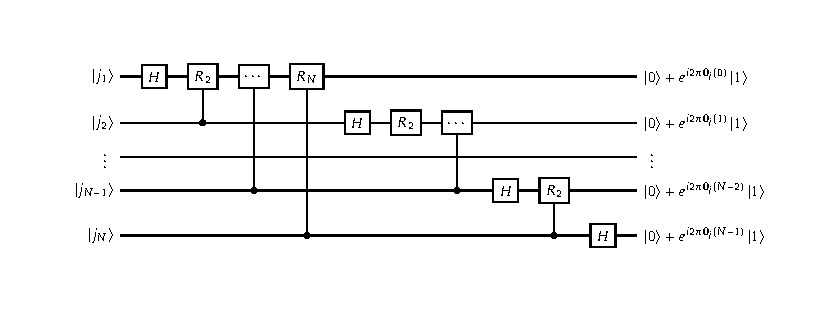
\includegraphics[width=0.9\textwidth]{Immagini/QFT.pdf}
    \caption
    {
        Circuits able to perform the quantum fourier tranform of the computational basis. It's important to notice how this algorithm is in reality not totally complete since the phases of the final states are inverted, so a series of swap gates needs to be inserted at the end to get the right form.
    }
    \label{fig:QFT}
\end{figure}
Now, this form of the QFT is much more usefull on an algorithmic point of view since it's now easy per us to see the operations that needs to be done on the single qubits. In particular, to reproduce the result we will need two types of gates that are also easy to understand that are
\begin{align}
    &H = \frac{1}{\sqrt{2}}\begin{pmatrix}
        1 & 1\\
        1 & -1
    \end{pmatrix},
    &R_k = \begin{pmatrix}
        1 & 0\\
        1 & e^{1\frac{2\pi}{2^k}}
    \end{pmatrix},
\end{align}
basically the Hadamart and phase gates. The final form of the circuit is described in \figref{fig:QFT}, where is possible to see how we can evaluate the QFT by the cimple use of controlled phase gates and swaps ones at teh end of the proces. This particular circuit is interesting since shows how quantum computers are able to perform fuorier transforms easily respect to classical algorithm. In fact, the number of gates required to perform such an operation scales as $\mathcal{O}(n^2)$ while the number of logic gates needed to perform the computation of a fast fourier transform inside a classical computer scales as $\mathcal{O}(n2^n)$. Quantum algorithm beats the classical one by an exponential factor. Nevertheless, the quantum algorithm has the big problem that the information are present in the phase of the states, and we are not able to evaluate them, basically meaning that the algorithm alone is useless. Still, we will see that QFT will still be used inside larger algorithm giving a lot of benefits.

\subsection{Phase evaluation}

The evaluation of phases inside quantum systems is always a troublesome problem, to the point that most of the time is thought as an impossible task. Nevertheless, is possible to see how the QFT algorithm is able to give us the possibility of experimentally evaluate a certain type of phase inside the system.

Let's imagine having a unitary operator $\mathcal{U}$ and wanting to evaluate the eigenvalues $\lambda_n$. We know from linear algebra that $\mathcal{U}\mathcal{U}^\dagger = \mathbb{1}$, so that from linear algebra we have the following information on the eigenvalues
\begin{align}
    &\lambda_n\lambda_n^* = \abs{\lambda_n}^2 = 1.
\end{align}
This relation tells us that the eigenvalues of such opeartors needs to be some kind of complex phases writable as
\begin{align}
    &\lambda_n = e^{2\pi i \phi_n}, &\phi_n \in [0, 1[.
\end{align}
Normally we would think that evaluating $\phi_n$ would be impossible since phases cannot be observed axperimentally. Still, we will show how using the eigenstate of the phases $\ket{u_n}$ and a simple operator $\mathcal{U}^{2^j}$ defined as follows
\begin{equation}
    \mathcal{U}^{2^j}: \ket{u_n} \longmapsto e^{2\pi i \phi_n 2^j} \ket{u_n},
\end{equation}
we are able to approximate its value with a wanted precision. In particular, we are aiming to approximate $\phi_n$ using a decimal form like the one in \eqref{eq:decimalForm}, so that we want to find $(b_n^1, b_n^2, \dots, b_n^t)$ so that 
\begin{equation}
    b_n = \frac{b_n^1}{2} + \frac{b_n^2}{4} + \dots + \frac{b_n^t}{2^t},
\end{equation}
is the decimal number $b < \phi_n$ closer to it as possible. Therefore, we are going to demonstrate that the algorithm showed in \figref{fig:Phase} is able to do exactly that, find out the values of $b_n^i$ approximating the phase up to a wanted accuracy.

\begin{figure}[t]
    \centering
    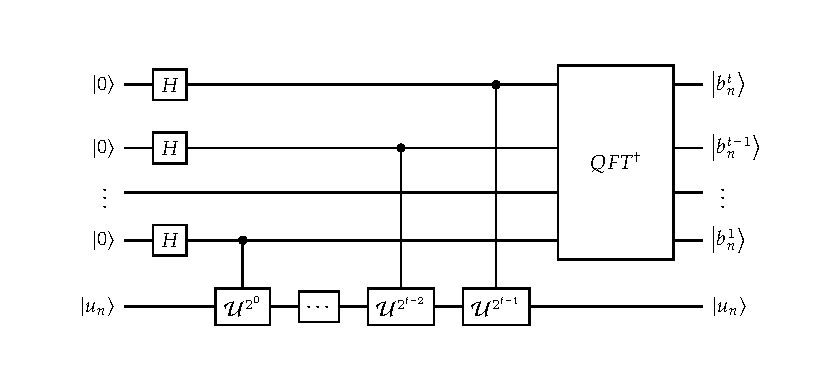
\includegraphics[width=0.8\textwidth]{Immagini/Phase.pdf}
    \caption
    {
        Quantum circuit for the approximation of the eigenvalues of a unitary operator up to a wanted accuracy based on the number of qubit used for the decimal approximation of the phase itself.
    }
    \label{fig:Phase}
\end{figure}

\thm{Phase evaluation}
{
    Taken a unitary operator $\mathcal{U}$ with eigenvalues defined by the phases $\phi_n$, the circuit \figref{fig:Phase} is able to give as output its decimal approximation $b_n$ with a wanted accuracy $\alpha > 0$, and precision $\epsilon > 0$ if the number of qubit used for the operation is
    \begin{equation}
        \label{eq:PhaseEvaluation}
        t > \alpha + \ln\left( 2 + \frac{1}{2\epsilon} \right).
    \end{equation}
}
\pf{Proof}
{
    First we need to look at what the circuit does effectivelly to the states, and it's easy to see that by looking at the case where $t = 1$ and see how the first part of the circuit works as follows
    \begin{equation}
        \left(C\mathcal{U}^{2^0}\right)\left(H\otimes\mathbb{1}\right)\ket{0}\otimes\ket{u_n} = C\mathcal{U}^{2^0}\left( \frac{\ket{0} + \ket{1}}{\sqrt{2}} \right)\otimes\ket{u_n} = \left( \frac{\ket{0} + e^{2\pi i\phi_n}\ket{1}}{\sqrt{2}} \right)\otimes\ket{u_n}.
    \end{equation}
    Which can be easily generalized to all the applications on the genearal $t$-dimensional circuit having a final form of the state given by
    \begin{equation}
        \ket{\psi_f} = \left[\bigotimes_{j = 0}^{t-1}\left( \frac{\ket{0} + e^{2\pi i\phi_n2^j}\ket{1}}{\sqrt{2}} \right)\right]\otimes\ket{u_n}
    \end{equation}
    Now, we know how every real number can be written as a converging series of rational numbers such as \eqref{eq:decimalForm} so that we are going to work with
    \begin{equation}
        \label{eq:rationalApproxPhase}
        \phi_n = \frac{\phi_n^1}{2} + \frac{\phi_n^2}{4} + \dots = \sum_{i=1}^\infty \frac{\phi_i}{2^i} \approx \sum_{i=1}^t \frac{\phi_i}{2^i}.
    \end{equation} 
    Meaning that can be approximated using the decimal representation described before, having that the phases can be rewritten using the following form
    \begin{equation}
        \exp\left( 2\pi i \phi_n 2^j \right) = \exp\left( 2\pi i\left\{ \left[ \phi_n^1 2^{j-1} + \dots \right] + \left[ \phi_n^{j+1}2^{-1} + \dots \right] \right\} \right) = \exp\left( 2\pi i \mathbb{0}_\phi(j) \right),
    \end{equation}
    where the first part was an integer giving no contribution. In this way one can understand that in the first part of the $\ket{\psi_f}$ state we end up having the QFT of the initial states, allowing us to write it in binary representation as
    \begin{equation}
        \ket{\psi_f} \approx \left( \frac{1}{2^{t/2}}\sum_{k=0}^{2^t-1}e^{2\pi i\phi_nk}\ket{k} \right)\otimes\ket{u_n}.
    \end{equation}
    In this way we can go and apply the inverse of the QFT and using the binary representation of the base to see what happens exactly in the transformation
    \begin{equation}
        QFT^\dagger \ket{\psi_f} = \frac{1}{2^t}\sum_{k=0}^{2^t-1} e^{2\pi i\phi_nk}\sum_{l=0}^{2^t-1} e^{-2\pi ikl/2^t}\ket{l} = \sum_l\left( \sum_{k=0}^{2^t-1}\frac{1}{2^t}e^{2\pi i (\phi_n - l/2^t)k} \right)\ket{l} = \sum_l c_l\ket{l}.
    \end{equation}
    The state becomes a superposition of states in the binary computational base of the $t$ qubits, and we know also the form of the coefficients. In fact, we can easily see how $c_l$ are composed by a geometric series giving rise to the following result
    \begin{equation}
        \label{eq:CoeffPhase}
        c_l = \frac{1}{2^t} \sum_{k=0}^{2^t-1} \left( e^{2\pi i (\phi_n - l/2^t)} \right)^k = \frac{1}{2^t}\frac{1 - e^{2\pi i (\phi_n - l/2^t)2^t}}{1 - e^{2\pi i (\phi_n - l/2^t)}}.  
    \end{equation}
    It's interesting to see how this result was obtained by truncating the real form of $\phi_n$ to a certain decimal order, but the procedure is general and works also in the case where the total series is retained. 
    
    Therefore, in \eqref{eq:CoeffPhase} the value of $\phi_n$ can be a rational or irrational number, and we can see what happens to $c_l$ in the two cases. In the case $\phi_n$ is rational we have that the approximation \eqref{eq:rationalApproxPhase} is exact, and we can write how
    \begin{equation}
        (\phi_n - l/2^t)2^t = \sum_{i=1}^t \phi_n^i 2^{t-i} -l = int.
    \end{equation}
    This means that the phase on the numerator of $c_l$ is a multiple of $2\pi$ and therefore $c_l = 0$ for every value of $l$ exept for $l=\phi_n 2^t$, where
    \begin{equation}
        c_{\phi_n2^t} = \frac{1}{2^t} \sum_{k=0}^{2^t-1} \left( e^{2\pi i (\phi_n - \phi_n)} \right)^k = \frac{2^t}{2^t} = 1.
    \end{equation}
    This means that $c_l = \delta_{l\phi_n2^t}$ which basically becomes a condition on the values of the single qubit that will take the following forms
    \begin{equation}
        \sum_{l=0}^{2^t-1} \delta_{l\phi_n2^t}\ket{l} = \ket{\phi_n2^t} = \ket{\phi_n^1}\otimes\ket{\phi_n^2}\otimes\dots\otimes\ket{\phi_n^t}, 
    \end{equation}
    where the binary representation was used to write down the single qubits. Now, we can simply evaluate all the $t$ qubits and have our approximation of the phase $\phi_n$ that is exact in this case, having that $b_n = \phi_n$.

    In the case $\phi_n$ is irrational, the truncation in the series generate an error having also that $(\phi_n - l/2^t)2^t$ is not an integer anymore and $c_l$ can be different from $0$ for other $l$ values. In this case we are going to approximate the value of $\phi_n$ using the values of $b_n$ that we obtain from the evaluation, and we want to know the error we are generating from such an approximation along with the accuracy of the result. Therefore, we select an error value $\omega$ and compute the probability of performing the measure 
    \begin{equation}
        \tilde{P} = P(\overline{l} \in [-\omega-1, \omega+1]),
    \end{equation}
    where $\overline{l} = l - \phi_n$ so that $\overline{l} = 0$ correspond to the real $\phi_n$. This evaluation can be performed using as $\omega$ the value $2^{t - \alpha} - 1$, where $\alpha$ is called accuracy, obtaining the result of
    \begin{equation}
        1 - \tilde{P} \le \frac{1}{2(2^{t-\alpha} - 2)}.
    \end{equation}
    Which identify the probability of not obtaining the wanted result, that we are going to set below a certain precision $\epsilon$ having $1 - \tilde{P}<\epsilon$ so that the following relations is found
    \begin{equation}
        t > \alpha + \ln\left( 2 + \frac{1}{2\epsilon} \right).
    \end{equation}
}
\noindent
Therefore, this algorithm is able to give us a really greate approximation for the phase that increase in accuracy as we scale up the number of qubit used in order to perform the operation. Also, it's possible to see how we from the inequality we can actually controll also the accuracy and precision of the prediction by setting them prior and then choose $t$ in order to satisfy \eqref{eq:PhaseEvaluation}.

\subsection{Grover algorithm}

Search algorithm are one of the most important type of algorithm that exist, since the aim is to find out specific elements inside a set that satisfy some requirements defined by ceratin function $f(x)$. Normally this kind of algorithms are really expensive scaling up real quick with both dimensions of the set and complexity of the function to use, but inside a quantum computer we can try to create a really efficient version of them.

Let's imagine to work with $n$ qubits, so that the computational base is composed by $N = 2^n$ elements that compose our set $\mathcal{N}$ in which only $1 \le M \le N$ elements are solutions of $f(x)$. Where, being solutions means that the state $\ket{x}$\footnote{We are using the binary representation for the state of the computational basis.} that represent that element is so that
\begin{equation}
    f(x) = \begin{cases}
        1 & x \in \text{solution}\\
        0 & x \notin \text{solution}
    \end{cases},
\end{equation}
basically $f: \mathcal{S} \to \{0, 1\}$ is a boolean function that gives true if it's solution and false otherwise. Then, we are going to need two types of gates that will generate the building blocks of our algorithm.
\thm{Oracle gate}
{
    The circuit shown in \figref{fig:oracle} is called oracle and is able to perform an inversion of the states that are not solution by using an ausiliary qubit in the $\ket{1}$ state.
    \begin{equation}
        \mathcal{O}\ket{x} = (-1)^{f(x)}\ket{x},
    \end{equation}
    so that if $\ket{x}$ is solution a $-1$ pops up, and remains equal otherwise.
}
\begin{figure}[t]
    \centering
    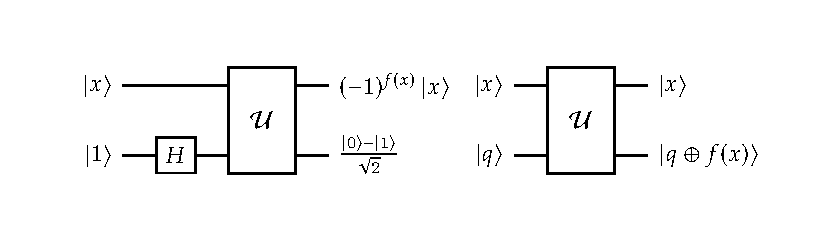
\includegraphics[width=0.8\textwidth]{Immagini/Oracle.pdf}
    \caption
    {
        Quantum circuit for the oracle gate used inside the algorithm to perform an inversion of the state about the components that are not solution to the function that we are interested in.
    }
    \label{fig:oracle}
\end{figure}
\pf{Proof}
{
    We can simply go over the different steps of the circuit to see how the following happens to the state
    \begin{equation}
        \mathcal{U}\left( \mathbb{1}\otimes H \right)\ket{x}\otimes\ket{1} = \mathcal{U}\ket{x}\otimes\left( \frac{\ket{0} - \ket{1}}{\sqrt{2}} \right) = \ket{x}\otimes\frac{1}{\sqrt{2}}\begin{cases}
            \ket{0} - \ket{1} & x \in \mathcal{S},\\
            \ket{1} - \ket{0} & x \in \mathcal{E}
        \end{cases}.
    \end{equation}
    Where $\mathcal{S}$ and $\mathcal{E}$ are the subset of $\mathcal{N}$ that contains the states that are solutions and not, respectivelly. Now, we can see how the difference between the two is simply a minus sign that we can imagine factorizing so that $\ket{x}$ takes it changing its phase as wanted.
}
\noindent
The next step is to define another type of gate that will be needed to perform another, more complex, type of reflection about the average state. Such gate is actually defined through also the use of a \textbf{conditional phase operator} defined as
\begin{equation}
    \mathcal{U}_x = 2\ketbra{x} - \mathbb{1},
\end{equation}
which has the effect of changing the phase to all state in the base that are not $\ket{x}$, and it's really easy to see since
\begin{align}
    &\mathcal{U}_x\ket{k} = \begin{cases}
        \ket{k} & k = x,\\
        -\ket{k} & k \neq x
    \end{cases}.
\end{align}
Using this idea we can define the wanted inversion operator in this particular way.
\thm{Inversion about the average}
{
    We can define the inversion about the average operator inside the space $\mathcal{N}$ as $\tilde{\mathcal{U}} = H^{\otimes n}\mathcal{U}_0 H^{\otimes n}$ and see how it's effect on a general state is
    \begin{align}
        &\ket{\phi} = \sum_{k\in\mathcal{N}}\alpha_k\ket{k}, &\tilde{\mathcal{U}}\ket{\phi} = \sum_{k\in\mathcal{N}}\left( 2\mean{\alpha} - \alpha_k \right) \ket{k}.
    \end{align}
    Which defines an inversion about the average state $\mean{\alpha}$.
}
\pf{Proof}
{
    We can first have a look at the form of the operator itself, which can be rewritten in a compact way as follows
    \begin{align}
        &\tilde{\mathcal{U}} = 2H^{\otimes n}\ketbra{0}H^{\otimes n} -\mathbb{1} = 2\ketbra{\psi} - \mathbb{1}, &\ket{\psi} = \frac{1}{\sqrt{N}}\sum_{k\in \mathcal{N}} \ket{k}.
    \end{align}
    Then, we can apply it to a general state to see how we retain the wanted result. In particular, we are going to write that
    \begin{align}
        &\tilde{\mathcal{U}}\sum_{k\in\mathcal{N}}\alpha_k\ket{k} = 2\sum_{k\in\mathcal{N}}\alpha_k\braket{\psi}{k}\ket{\psi} - \sum_{k\in\mathcal{N}}\alpha_k\ket{k} = 2\sum_{k\in\mathcal{N}}\sum_{l\in\mathcal{N}}\sum_{x\in\mathcal{N}}\frac{\alpha_k}{N} \braket{l}{k}\ket{x} - \sum_{k\in\mathcal{N}}\alpha_k\ket{k},
    \end{align}
    where we can use the fact that $\braket{l}{k} = \delta_{lk}$ to eliminate a summation and then see how $\sum_{k\in\mathcal{N}}\alpha_k/N = \mean{\alpha}$ so that the final result is obtained as
    \begin{equation}
        \tilde{\mathcal{U}}\sum_{k\in\mathcal{N}}\alpha_k\ket{k} = 2\sum_{x\in\mathcal{N}}\mean{\alpha}\ket{x} - \sum_{k\in\mathcal{N}}\alpha_k\ket{k} = \sum_{k\in\mathcal{N}}\left( 2\mean{\alpha} - \alpha_k \right) \ket{k}.
    \end{equation}
}

These two gates are the building blocks that will allow us to perform the quantum search and the idea to that is to actually define an operator that will allow us to transform the state into a linear combination of the ones that are solutions to our function. This can be done easily, since the following result holds, giving us the final form for the quantum search algorithm.
\thm{Quantum search}
{
    A general state $H^{\otimes n}\ket{0}$ can be decomposed in two main parts inside $\mathcal{N}$ as
    \begin{equation}
        \ket{\psi} = H^{\otimes n}\ket{0} = \sin\frac{\theta}{2}\ket{\beta} + \cos\frac{\theta}{2}\ket{\alpha},
    \end{equation}
    where $\ket{\beta}$ is a linear combination of all the solutions of $f(x)$, while $\ket{\alpha}$ a combination of all the non-solutions. The \textbf{Groover opeartor} $\mathcal{G} = \tilde{\mathcal{U}}\mathcal{O}$ acts on this state by rotating the angle $\theta$ in the direction of $\ket{\beta}$, so that if applied $R$ times we get
    \begin{equation}
        \mathcal{G}^R\ket{\psi} = \sin\left( \frac{2R + 1}{2}\theta \right)\ket{\beta} + \cos\left( \frac{2R + 1}{2}\theta \right)\ket{\alpha}.
    \end{equation}
    Therefore, we can select the right number of $\mathcal{G}$ to perform in order to obtain the maximum likelihood to obtain as a result of the measurament the state $\ket{\beta}$ with the solutions of the function.
}
\begin{figure}[t]
    \centering
    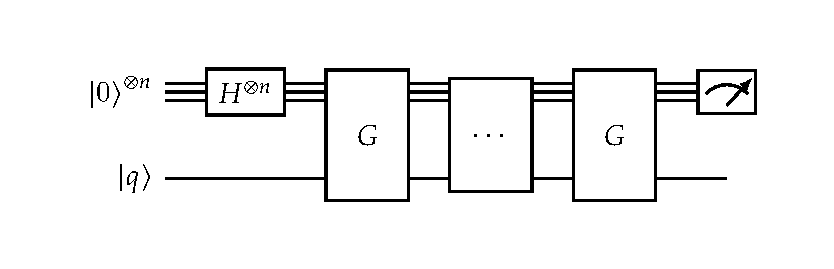
\includegraphics[width=0.7\textwidth]{Immagini/Groover.pdf}
    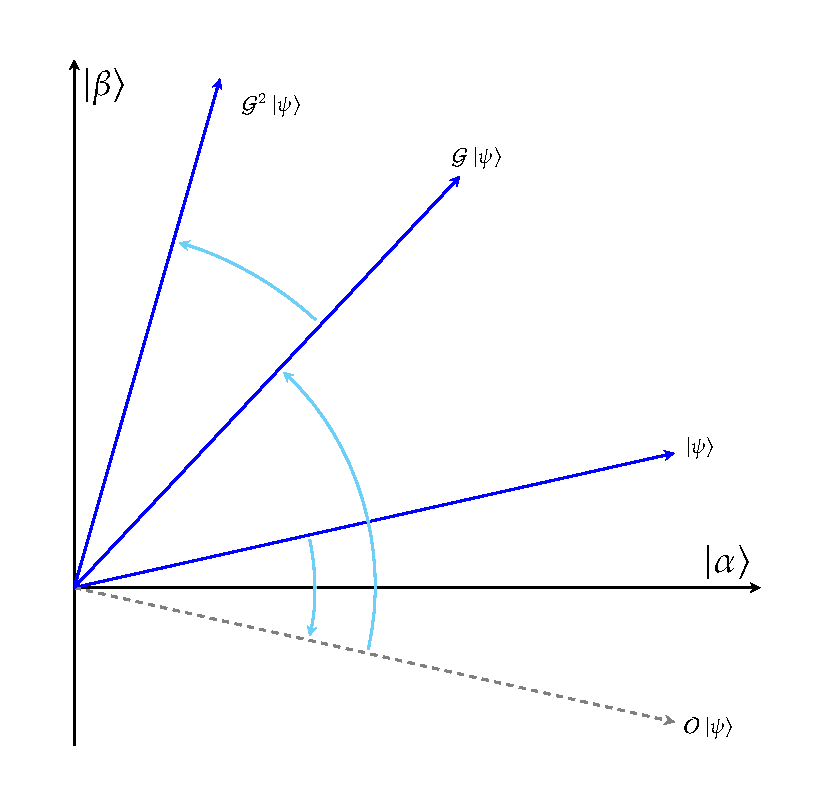
\includegraphics[width=0.25\textwidth]{Immagini/TrasfGrov.pdf}
    \caption
    {
        Graphical representation of the Groover's circuit, to the left, with transformations that happens to the state in the quantum search algorithm, to the right, in order to understand how the two reflection tranforms into a rotation.
    }
    \label{fig:Groover}
\end{figure}
\pf{Proof}
{
    We can start by looking at the general state $\ket{\psi}$ and see how can be rewritten as linear combination of solution and non-solution as follows
    \begin{equation}
        \ket{\psi} = \frac{1}{\sqrt{N}}\left( \sum_{k\in \mathcal{S}}\ket{k} + \sum_{k\in\mathcal{E}}\ket{k} \right) = \sqrt{\frac{M}{N}}\left( \frac{1}{\sqrt{M}}\sum_{k\in \mathcal{S}}\ket{k} \right) + \sqrt{\frac{N-M}{N}}\left( \frac{1}{\sqrt{N-M}}\sum_{k\in \mathcal{E}}\ket{k} \right),
    \end{equation}
    now we can see how $\sqrt{M/N}$ and $\sqrt{N-M/N}$ can be setted as the sine and cosine, while the superpositions that are mulitpling are exactly the linear combinations of all solutions and non-solutions respectivelly. Therefore, we effectivelly have that the following is true
    \begin{align}
        H^{\otimes n}\ket{0} = \sin\frac{\theta}{2}\ket{\beta} + \cos\frac{\theta}{2}\ket{\alpha},
    \end{align}
    then we shall see what the operator $\mathcal{G}$ does on it, and that can be done by looking at $\mathcal{O}$ and $\tilde{\mathcal{U}}$ separatelly. First, it's easy to understand how the oracle gate simply changes the sign of the $\ket{\beta}$ coefficient, meaning that using it simply performs a reflection of the state respec to the $\ket{\alpha}$ one. Then, the inversion by the average operator instead perform another inversion in this case that is respect to the state $\ket{\psi}$, so that two inversions apply one after giving a final rotation of the state as
    \begin{equation}
        \mathcal{G}\ket{\psi} = \sin\left( \frac{3}{2}\theta \right)\ket{\beta} + \cos\left( \frac{3}{2}\theta \right)\ket{\alpha},
    \end{equation}
    which is also depicted in \figref{fig:Groover}. Meaning that the rotation allowed for the state to become closer to the $\ket{\beta}$ state, and if we continue to perform it we will get as a state
    \begin{equation}
        \mathcal{G}^R\ket{\psi} = \sin\left( \frac{2R + 1}{2}\theta \right)\ket{\beta} + \cos\left( \frac{2R + 1}{2}\theta \right)\ket{\alpha}.
    \end{equation}
    In this way we can see how the probabilities of having as result $\ket{\beta}$ scales up since the angle gets closer to $\pi/2$, which gives $1$ as coefficient for that state. Still, it's possible to do too many rotations and ending up to go past the perfect value and increasing the coefficients for the $\ket{\alpha}$ state, still one can see how if $R$ is choosen as
    \begin{align}
        &R = \left[ \frac{\arccos\sqrt{M/N}}{\phi} \right], &\phi \le 4,
    \end{align}
    where $\left[ x \right]$ is the integer part function, we will have probabilities that looks like
    \begin{align}
        &P_\beta > 1/2, &P_\alpha < 1/2.
    \end{align}
    Basically, we can select $\phi$ to obtain the most optimized result possible, and already we know that by default the probabilities are in favor of the right result that we are serching for.
}
\noindent
Therefore, this algorithm allows us to search inside a set of states of dimensions $2^n$ the ones that satisfy the condition imposed by a wanted function $f$. Also, all of this is done by using a minimal number of operations that scales linearly with the number of qubit that we are using, beating in an increadible way the classical search algorithm that scales exponentially.

\subsection{Hamiltonian simulation}

On of the main goals that quantum computers scientists whant to achive is the possibility of simulate complex quantum systems efficiently thanks to the intrinsic quantum nature of QC themselfes. Basically the goal is to find a way to solve the SE inside a quantum computer finding out the time evolution operator of the system, which we recal in a time-independent $\mathcal{H}$ is
\begin{align}
    &\ket{\psi(t)} = \mathcal{U}(t)\ket{\psi_0}, &\mathcal{U}(t) = \exp\left( -i \frac{\mathcal{H}t}{\hbar} \right).
\end{align}
In order to do that we shall approximate the form of $\mathcal{U}(t)$ somehow using the qubit that we have avaliable, and the idea is the one of discretize it along with also $\ket{\psi}$. Basically, $\ket{\psi}$ will be thought as a function $\psi(\vb{x})$ where $\vb{x}\in\mathbb{R}^d$, and we are going to store only a set of values, of that function defined by the position on a lattice $\{x_j\}_j$, inside the qubit. Such discretization, then, nedds to be used also for the Hamiltionan, having an approximate form also for it, which define the evolution operator that we can then use to evolve the state.

To understand better how this is done we will assume that $\mathcal{H}$ is composed by a series of smaller components $\mathcal{H}_k$ containing only short range interactions, like
\begin{align}
    &\mathcal{H} = \sum_{k=1}^L \mathcal{H}_k = \sum_{\langle nm \rangle} Z_nZ_m +h\sum_l\left( Z_l + X_l \right).
\end{align}
This is an Ising Hamiltonian that has only on-site terms with longitudinal and trasversal field, and an interaction term that still applies only on nierest neighbours. Basically, we assume that $\mathcal{H}_k$ has interaction that at most account for a finite number of elements near a particular qubit. Inside these assumptions we can easily go and find out a way to approximate evolution operator by using a Taylor expansion as
\begin{equation}
    \label{eq:EasyApprox}
    \mathcal{U}(\Delta t) = \sum_{k=0}^\infty \frac{1}{k!}\left( -i\frac{\mathcal{H}\Delta t}{\hbar} \right)^k = \mathbb{1} - i\frac{\mathcal{H}\Delta t}{\hbar} + \mathcal{O}(\Delta t^2),
\end{equation}
where $\Delta t$ is the time discretization, assumed to be small. Also, from this poin on we will assume $\hbar = 1$ for simplicity of notation. We can see how the sum can be truncated to obtain an approximation of $\mathcal{U}$ that becomes better as the time discretization goes down, which is greate but not too greate. A better approach would be taking advantage of the decomposition of the Hamiltionian in pieces in order to rewrite the exponential as product of simpler operators that we know how to work with. Nevertheless, it's easy to see how also in the simple case we have looked at the $\mathcal{H}_k$ does not commute $\left[ \mathcal{H}_k, \mathcal{H}_m \right] \neq 0$, meaning that
\begin{equation}
    \exp\left( -it\sum_k\mathcal{H}_k \right) \neq \prod_{k}\exp(-it\mathcal{H}_k).
\end{equation}
This seems to set the sloppy \eqref{eq:EasyApprox} as the only possible way to approximate the operator, but it's not completely true. In fact, it's possible to demonstrate a result that saves the day.
\thm{Trotler decomposition}
{
    Taken two non commuting operators $A, B$ it's possible to decompose the exponential in the following way
    \begin{equation}
        \exp\left[ i\left( A + B \right)t \right] = \lim_{N\to\infty}\left( e^{i\frac{t}{N}A}e^{i\frac{t}{N}B} \right)^N.
    \end{equation}
}
\pf{Proof}
{
    We can use \eqref{eq:EasyApprox} to write down the following form
    \begin{equation}
        e^{i\frac{t}{N}A}e^{i\frac{t}{N}B} = \left[ \mathbb{1} - i\frac{\Delta t}{N}A + \mathcal{O}(1/N^2) \right]\left[ \mathbb{1} - i\frac{\Delta t}{N}B + \mathcal{O}(1/N^2) \right] = \mathbb{1} + i\frac{t}{N}\left( A + B \right) + \mathcal{O}(1/N^2),
    \end{equation}
    which elevated to the power of $N$ allow for the following result to show up
    \begin{equation}
        \left( e^{i\frac{t}{N}A}e^{i\frac{t}{N}B} \right)^N = \mathbb{1} + \sum_{K=1}^N \binom{N}{k}\frac{\left[ it\left( A + B \right) \right]^k}{N^k} + \mathcal{O}(1/N). 
    \end{equation}
    Here, is possible also to see how the binomial coefficents can be approximated in the following way
    \begin{equation}
        \binom{N}{k} \frac{1}{N^k} \sim \frac{1}{k!} + \mathcal{O}(1/N),
    \end{equation}
    having that the final form becomes exactly the sum of the Taylor expansion wanted in the limit of $N\to\infty$.
}
\noindent
Such a result allows for a better way to approximate the evolution operator by setting a ceratin discretization defined by $N$ and then perform several steps in the middle. This can be also done analitically to find out some important closed formulas in order to have a better computational approach, and the most used one is the \textbf{Baker Hausdorff formula}
\begin{equation}
    e^{i(A+B)\Delta t} = e^{iA\Delta t}e^{iB\Delta t} e^{-\frac{i}{2}[A, B]\Delta t^2} + \mathcal{O}(\Delta t^3).
\end{equation}
Which is a good improvment of the previous naive approximation.

Let's now imagine that we want to work in order to simulate a 1D particle inside a potential $V(x)$, we will have that the system is described as
\begin{align}
    &\mathcal{H} = \frac{\hat{p}^2}{2m} + V(\hat{x}), &x\in [-d, d].
\end{align}
In this situation we discretize the space to have a spacing $a = 2d/N$ and the points on the lattice that we are working with are described by the values
\begin{align}
    &x_j = aj, &j\in\left[ -N/2, N/2 \right].
\end{align}
In this way we will define the position basis as the set $\{x_j\}$ so that the following is true 
\begin{equation}
    V(\hat{x}) \ket{x_j} = V(x_j) \ket{x_j},
\end{equation}
having that they diagonalize the potential part of the Hamiltonian. Using this base also the state of the particle can be written as a linear combination of the type
\begin{equation}
    \ket{\psi} = \sum_{j = -N/2}^{N/2} \alpha_j \ket{x_j}.
\end{equation}
Therefore, this set allows for the discretization of both the state of the particle and a part of the Hamiltonian, to complete our needs we will need also to store the momentum part of the Hamiltonian, but it's not diagonal in such base. For this reason, the idea is to write $\hat{p}$ as the Fourier transform of the position operator $\mathcal{U}_{FT}\hat{x}\mathcal{U}_{FT}^\dagger$ since we know to perform the Fourier tranform of the state, meaning that we can effectivelly evaluate also $\hat{p}\ket{x_j}$ having all that we need.

\begin{figure}[t]
    \centering
    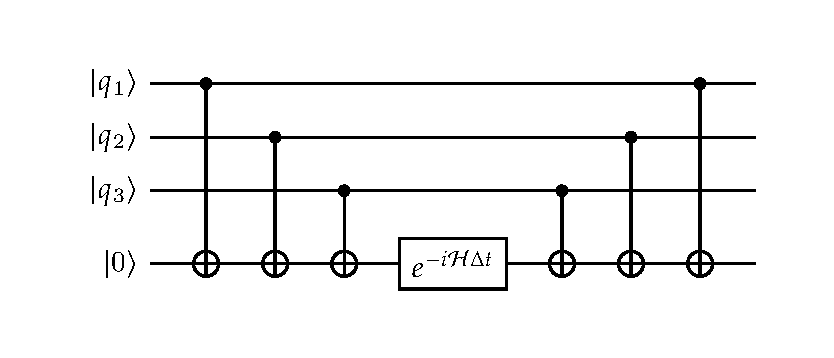
\includegraphics[width=0.8\textwidth]{Immagini/HSim.pdf}
    \caption{
        Quantum circuit used in order to simulate the simple system of the example, if the circuitis folled it's effectivelly possible to see how the final form is exactly the initial state plus the wanted phase and the ancilla qubit.
    }
    \label{fig:HSim}
\end{figure}

\ex{Simple case}
{
    The prof showed a really simple example of system simulation on a quantum computer, where the Hamiltonian is simply 
    \begin{equation}
        \mathcal{H} = Z_1\otimes Z_2\otimes Z_3,
    \end{equation}
    meaning that three qubit are studied and the base is so $\ket{q_1q_2q_3}$. We shall also remember that the effect of $Z$ is changing sign to the state if it's value is $1$ or not touching it otherwise. Knowing it allows us to find out how the Hamiltonian act on a general state having
    \begin{align}
        &\mathcal{H}\ket{q_1q_2q_3} = \delta_{q_1q_2q_3}\ket{q_1q_2q_3}, &\delta_{q_1q_2q_3} = \begin{cases}
            1 & \#1\text{ is even},\\
            -1 & \#1\text{ is odd}
        \end{cases}.
    \end{align}
    Using this we can implement a quantum circuit that simulates the evolution by adding the correct phase to a general state of the base every time is applied to it. The circuit we are talking about is represented in \figref{fig:HSim}, where one can see how the ancilla qubit will be $1$ befor the phase gate if an odd number of 1 are present in the initial state, and then will return to the initial state. Therefore, the final result is simply $e^{i\delta\Delta t}\ket{q_1q_2q_3}\otimes\ket{0}$, the state has effectivelly evolved as we wanted.
}
    \section{Universality of quantum computation}

An important property that we want to obtain inside ours computer is the universality of the logic we are using. Meaning that we aim in being able to represent all the possible function using only a restricted number of operations in order to implement only those inside our machine, making the implementation much easier. In order to demonstrate it inside quantum computers we need first to make this concept more formal, aiming so to a definition like the following.
\dfn{Universality}
{
    A type of computation is universal if exist a small set of gates that can be used to write any algorithm.
}
\noindent
We know how classical computations have such properties since it's possible to demonstrate how all the ingredients that are needed to compose every circuit are the following:
\begin{enumerate}[label*=\protect\fbox{\arabic{enumi}}]
    \item Wires, connecting different gates conserving states;
    \item Ancilla bits, in order to do more complex operations;
    \item FANOUT to duplicate the state of a bit;
    \item CROSSOVER swapping states between bits;
    \item AND, XOR and NOT gates able to generate all the others.
\end{enumerate}
It's also possible to use only the NAND gate to similate all of AND, XOR and NOT being the universal gate of classical logic.

What we want to do is see how the following components are also what we need inside quantum computations to be universal, and components from 1 to 4 are already given to us by discussions in precedent sections. Therefore, all remains is to see if exist a set of gates that allow us to write down all possible unitary operations doable on a set of qubit.

\subsection{Gates decomposition}

To see how to recreate universality we need to see if a general gate $\mathcal{U}$ acting on $n$ qubit, so a general $2^n\times 2^n$ unitary matrix, can be decomposed in several similar operations. This is duable using the concept of two-level gate defined as.
\dfn{Two-level gates}
{
    A gate is defined to be two-level if leaves invariant $2^n - 2$ states and modify in a non-trivial way the remaining two. Basically, acts only on two specific states.
}
\noindent
Using such gates we can write down all possible unitary matrices and this can be seen in the following result
\thm{Two-level universality}
{
    Every unitary matrix $\mathcal{U}$ with dimension $d\times d$ can be decomposed using at most $\mathcal{O}(2^{2n})$ two-level gates.
}
\pf{Proof}
{
    We haven't really seen a rigourus proof of such a statement we have only worked out the case with $d = 3$. Let $\mathcal{U}$ be a generally $3\times 3$ unitary matrix as
    \begin{equation}
        \mathcal{U} = \begin{pmatrix}
            a & b & c\\
            d & e & f\\
            g & h & i
        \end{pmatrix},
    \end{equation}
    we can choose some two-level opeartions to perform depending on its values. In particular, we choose
    \begin{align}
        &\text{if }d=0 \hspace{0.5cm}\mathcal{U}_1 = \begin{pmatrix}
            1 & 0 & 0\\
            0 & 1 & 0\\
            0 & 0 & 1
        \end{pmatrix}, &\text{if }d\neq 0 \hspace{0.5cm}\mathcal{U}_1 =\begin{pmatrix}
            \frac{a^*}{\sqrt{\abs{a}^2 + \abs{b}^2}} & \frac{b^*}{\sqrt{\abs{a}^2 + \abs{b}^2}} & 0\\
            \frac{b}{\sqrt{\abs{a}^2 + \abs{b}^2}} & -\frac{a}{\sqrt{\abs{a}^2 + \abs{b}^2}} & 0\\
            0 & 0 & 1
        \end{pmatrix}.
    \end{align}
    In this way it's possible to see how mutipling the two unitary matrices one can obtain the following result
    \begin{equation}
        \mathcal{U}_1\mathcal{U} = \begin{pmatrix}
            a' & b' & c'\\
            0 & e' & f'\\
            g' & h' & i'
        \end{pmatrix},
    \end{equation}
    an element of the matrix was setted to $0$. We can then go on and use another transformation in a way similar to the one before as
    \begin{align}
        &\text{if }c'=0 \hspace{0.5cm}\mathcal{U}_2 = \begin{pmatrix}
            a'^* & 0 & 0\\
            0 & 1 & 0\\
            0 & 0 & 1
        \end{pmatrix}, &\text{if }c'\neq 0 \hspace{0.5cm}\mathcal{U}_2 =\begin{pmatrix}
            \frac{a'^*}{\sqrt{\abs{a'}^2 + \abs{c'}^2}} & 0 & \frac{c'^*}{\sqrt{\abs{a'}^2 + \abs{c'}^2}}\\
            0 & 1 & 0\\
            \frac{c'}{\sqrt{\abs{a'}^2 + \abs{c'}^2}} & 0 & -\frac{a'}{\sqrt{\abs{a'}^2 + \abs{c'}^2}}
        \end{pmatrix}.
    \end{align}
    Applied it we can see how the matrix simply further becoming simply
    \begin{equation}
        \mathcal{U}_2\mathcal{U}_1\mathcal{U} = \begin{pmatrix}
            1 & b'' & c''\\
            0 & e'' & f''\\
            0 & h'' & i''
        \end{pmatrix},
    \end{equation}
    but due to unitary constrain also $b'' = c'' = 0$ meaning that we can simply finish the work by using the inverse $\mathcal{U}_3$ that is a two-level unitary matrix and have that
    \begin{equation}
        \mathcal{U}_3\mathcal{U}_2\mathcal{U}_1\mathcal{U} = \mathbb{1},
    \end{equation}
    leaving us with the fact that $\mathcal{U}_3\mathcal{U}_2\mathcal{U}_1 = \mathcal{U}^\dagger$, reconstructing the full matrix using simple two-levels opeations. It's easy to understand how the process can be scaled up to whatever dimension of the matrix allowing for the decomposition in two-level opeartions of all possible gates. We can also have an estimate of the number of operations inside such a decomposition and the idea is that for a $d$ dimensional matrix you need at most $d-1$ opeartions to eliminate the first row and have a $d-1$ matrix, then $d-2$ opeartions needs to be done for reducing it further and so on having at most a complexity of
    \begin{equation}
        (d-1) + (d-2) + \dots + 1 = \frac{d(d-1)}{2}.
    \end{equation}
    Taking into account that inside a quantum computer $d = 2^n$ we will have $\mathcal{O}(2^{2n})$ as complexity. 
}
\noindent
Basically we have demonstrated o how two-level gates are universaly able to represent every possible gate taht we can imagine inside a quantum computer.

We can then go further, since the set of two-level gates is infinite, and we can't imagine implementing an infinite number of gates inside a software to reproduce all possible gates. In fact, we can restict our view simply to the set of CNOT, that we will use to implement the SWAP, and of single-qubit gates meaning that we manipulate only a single qubit.
\thm{CNOT and single qubit universality}
{
    Every two-level gate can be decomposed in a series of CNOT operations followed by a single qubit manipulation.
}
\pf{Proof}
{
    Basically we can imagine every two-level gate as a particular unitary matrix with all one on the diagonal and four coeffients around inside it needed to manipulate the two-states designed, similar to the one seen in the previous demonstration. We want to rewrite such a trasnformation simply using swap operations, that can be seen as permutations of the states, and a single qubit operations that can be written as
    \begin{equation}
        \tilde{\mathcal{U}} = \begin{pmatrix}
            1 & \dots & \dots & \dots & \dots & 0\\
            \vdots & \ddots & & & & \vdots\\
            \vdots & & a & b & & \vdots\\
            \vdots & & c & d & & \vdots\\
            \vdots & & & & \ddots & \vdots\\
            0 & \dots & \dots & \dots &\dots & 1
        \end{pmatrix}.
    \end{equation}
    To see this we can make an example with a $4\times 4$ matrix bacting in the following way. The matrix $\mathcal{U}$ we are working with is the following 
    \begin{equation}
        \mathcal{U} = \begin{pmatrix}
            a & 0 & b & 0\\
            0 & 1 & 0 & 0\\
            c & 0 & d & 0\\
            0 & 0 & 0 & 1
        \end{pmatrix},
    \end{equation}
    what we need to do is first see how we can swap the states, meaning that by using a permutation we can change the column and the rows of the matrix as if we are chaning the base of computation. In this way by using the permutations that bring $\ket{10}$ to $\ket{01}$, meaning the SWAP gate composed on CNOT in \eqref{eq:swapMatrix}, and see how the following it's true
    \begin{equation}
        SWAP(\ket{01}\to \ket{10})^\dagger\mathcal{U}SWAP(\ket{01}\to \ket{10}) = \begin{pmatrix}
            a & b & 0 & 0\\
            c & d & 0 & 0\\
            0 & 0 & 1 & 0\\
            0 & 0 & 0 & 1
        \end{pmatrix},
    \end{equation}
    which is simply a single qubit gate and inverting the operation we can see how $\mathcal{U}$ can be written with two swaps and a $\tilde{\mathcal{U}}$ operation. On a much larger scale the idea is to perform a series of swap to bring the state close together forming a single qubit operation, do that, and then reswap the states to return to the original form. This approach is called \textbf{gray code} algorithm and allows to generally write down every two-level operation as one single qubit one and $2(n-1)$ swaps at most, where $n$ is the number of qubit.
}
\noindent
Thanks to this last result we can say that the all set of the two-level operation can be reduced further to the one comprhending CNOT and single qubit operations, much smaller and simpler to implement inside a real quantum computer. Also, we can make an estimate of the total number of operations needed in order to recreate exactly a particular gate $\mathcal{U}$ inside a quantum computer composed by $n$ qubit. In fact, we have that every opeartion can be written as, at most, $2^{2n}$ two-level operation and every one of them need a $\tilde{\mathcal{U}}$ and $2(n - 1)$ swaps giving a total complexity of
\begin{equation}
    \mathcal{O}(n^22^{2n}),
\end{equation} 
which is quite highy but allows to have an exact result for every possible operation.

\subsection{Single qubit gates approximation}

We have seen how in order to decompose every possible gate inside a quantum computer we need the CNOT one and all the single qubit operartion that we can perform. Still, the latter have infinite possibilities inside quantum computers, and we can't implement all of that on a hardware level. For this reason, we want to create a small finite set of operation that can reproduce all of them also in an approximate way.

The idea is to find out a set of operations that allow us to find out a $\mathcal{V}$ that minimize the error in the estimate of the real $\mathcal{U}$, where the error is defined as
\begin{equation}
    E[\mathcal{U}, \mathcal{V}] = \max_{\ket{\psi}}\left\lVert \left( \mathcal{U} - \mathcal{V} \right)\ket{\psi} \right\rVert. 
\end{equation}
There are a several way in which such a minimization can be done using varius set of opeartor but the most used one is the standard composed by the following
\begin{equation}
    \mathcal{S} = \{H, CNOT, T\}.
\end{equation}
Only those three gates will be able to create every possible operation inside a quantum computer. In particular, we need to demonstrate that we are able to generate all the single qubit gate up to a certain error using them, and can be seen as follows.
\thm{$T$ and $H$ universality}
{
    Let $R_{\vb{n}}(\theta)$ be a generic roation of the single qubit state, where $\vb{n}$ is the versor that defines the roation and $\theta$ the angle of the rotation. Then for every $\epsilon > 0$ exist a $\vb{m} \in \mathbb{N}^3$ so that by defining $R_T = THTH$ we will have
    \begin{equation}
        E[R_{\vb{n}}(\theta), R_T^{m_1} HR_T^{m_2}H R_T^{m_3}] < \epsilon.
    \end{equation}
}
\pf{Proof}
{
    Also here we haven't done a real demonstration of the result, but still we can see the main reasons why that works. The idea is to first recall that every rotation can be written as
    \begin{equation}
        \label{eq:UniversalApprox}
        R_{\vb{n}}(\theta) = \exp\left( -i\frac{\theta}{2}\vb{n}\vdot \vb*{\sigma} \right) = \cos\left( \frac{\theta}{2} \right)\mathbb{1} - i\sin\left( \frac{\theta}{2} \right)\vb{n} \vdot \vb*{\sigma},
    \end{equation}
    and then look at how the operator $R_T$ look like by writing it down explicitly. To do that we need first to recall two things
    \begin{align}
        &T = \exp\left( -i\frac{\pi/4}{2}Z \right), &HTH = \exp\left( -i\frac{\pi/4}{2}X \right),
    \end{align}
    so that we can easily write down the wanted rotation as
    \begin{equation}
        R_T = \exp\left( -i\frac{\pi/4}{2}Z \right)\exp\left( -i\frac{\pi/4}{2}X \right) = \cos^2\left( \frac{\pi}{8} \right)\mathbb{1} - i\left[ \cos\frac{\pi}{8}\left( X + Z \right) + \sin\frac{\pi}{8} Y \right]\sin\left( \frac{\pi}{8} \right).
    \end{equation}
    Such thanks to the properties of the special angle $\pi/8$ such operator defines exactly a rotation respect to a particular versor $\tilde{\vb{n}}$ and angle $\tilde{\theta}$ defined by
    \begin{align}
        &\tilde{\vb{n}} = \frac{\left( \cos\frac{\pi}{8}, \sin \frac{\pi}{8}, \cos \frac{\pi}{8} \right)}{\sqrt{2\cos^2\frac{\pi}{8} + \sin^2\frac{\pi}{8}}}, &\cos \frac{\tilde{\theta}}{2} = \cos^2\frac{\pi}{8}.
    \end{align}
    Now, this is really good since the angle $\tilde{\theta}$ is irrationale meaning that for every angle $\phi \in [0, 2\pi]$ and $\epsilon > 0$ exist an integer $m$ so that
    \begin{equation}
        \abs{\phi - \left\lVert m\tilde{\theta} \right\rVert_{2\pi} } < \epsilon,
    \end{equation}
    where here $\left\lVert \vdot \right\rVert_{2\pi} $ indicates the module of $2\pi$. Meaning that we are able to came close to every possible angle of rotation that we want in this contest. In this way we can understand how the relation in \eqref{eq:UniversalApprox} holds true in general so that a single qubit gate can be approximated using in general a $\mathcal{O}(m^2/\epsilon)$ number of gates.
}
\noindent
That's it, we have demonstrated how by using a set composed by only three gates we are able to generate universally every possible operation that we can imagine, and that is exactly what happens inside a quantum computer. If you give as imput to the computer to perform a rotation of $\pi/9$ in reality he is decomposing it in a series of $\pi/8$ and hadamart gate to approximate it to a ceratin precision.

In reality exist a much more rich theory that allows us to give a better approximation that we have only cited during the course and is the following.
\thm{Solovay-Kitaev theorem}
{
    An arbitrary single qubit gate can be approximated to an accuracy $\epsilon$ using at most
    \begin{align}
        &\mathcal{O}\left(\log^c\frac{1}{\epsilon}\right), &c \sim 2.
    \end{align}
}
\noindent
Meaning that if we need $m$ CNOT and $m$ single qubit gates we will have a final complexity for the operation given by $\mathcal{O}\left( m\log^c(m/\epsilon) \right)$, not bad at all.
    \section{Quantum error coorection}

It's perfectly known how computers are affected from machine errors, where bits can possibly change states due to various external factors. The same thing happens to quantum computers, in paticular qubits are much more delicate having a greate number of possible fluctuations that needs to be taken into account when we run an algorithm. Therefore, we need to create protocols that allow us to correct such variations of the state during the computations as we have inside classical computers. In order to understand how this can be done on a quantum level is really usefull to see its classical version and grasp the major concepts to use also on quantum computers.

On classical computers a bit can change state randomically going from $0$ to $1$ or viceversa with a certain probability $p$ inside the circuit. Such a situation define a particular type of transformation that we will define as follows.
\dfn{Binary symmetric channel}
{
    When we will have a transformation $X:\{0,1\} \to \{0,1\}$ acting on the state of a logic variable so that $X(0) = 1$ with a certain probability $p$ and $X(0) = 0$ with $1-p$ it's called binary symmetric channel.
}
\noindent
Such are the randomic trasnformation that acts on the single bits inside a normal computer, having that they can be overcomed using a regular routine that has becomed standard over the years. The idea is the following, we are going to \textbf{encode} the state of a single bit using three of them such as follows
\begin{align}
    &0 \mapsto 000, &1\mapsto 111.
\end{align}
In this way we will have that an error on one the bits defining the state can be \textbf{dyagnosed} by looking at the other two. In particular, we will have that if we start from $000$ and on the line we see a $100$ we know that an error has occoured, and we are able to correct it. We know how the possible flips that could have happened bringing to the $100$ are: a flip to the first bit in the state $000$, and two bits flips for second and third in the $111$ state. In this context, in order to \textbf{recover} the state, the idea is to return to the state that has the higher probability of being the right one, in the situation we have discussed is the $000$ since we have a probability $p$ of flipping to that state while $111$ has a probability $p^2$. Such a protocol, called \textbf{majority rate}, allows to brign the possibility of the error to propagate inside the circuit to the one given by the following result.
\thm{Majority rate error probability}
{
    The probability of committing an error by using the majority rate protocol is given by
    \begin{equation}
        \label{eq:ErrMajoRate}
        p_{err} = 3p^2 - 2p^3.
    \end{equation}
}
\pf{Proof}
{
    In the protocol we are basically ignoring the possibilities of having more than one flip, so tha tthe error is given by the possibility of having every two flip or a three bit flip, giving
    \begin{equation}
        p_{err} = 3p^2(1-p) + p^3 = 3p^2 - 2p^3.
    \end{equation}
}
\noindent
It's also interesting to see how such a simple protocol is also not always usefull. In fact, the inequality $3p^2 - 2p^3 < p$ is true only if $p < 1/2$ or the opposite is real, having that such an error correction can be used only if the probability of error of a single bit is already bellow that threshold.

This was a simple protocol, but it still shows the main important features that a general error correction code should have in principle. We can sintetyze what is needed in order to correct the error on an abstract level as: encoding of the state, dyagnosis of the error committed, and recover of the original state. All of this is not difficult to imagine done inside a normal computer, still working with quantum information makes thing a lot harder due to the presence of some complications:
\begin{enumerate}[label*=\protect\fbox{\arabic{enumi}}]
    \item The no cloning theorem makes diffucult coping the state, having that encoding is not too much straightforward;
    \item The types of errors inside a qubit are larger than the simple flip of a bit, in fact we have the whole range of continuos unitary transformation to span;
    \item Recover a state it's not easy to do expecially remembering that if we measure a state we are going to lose it forever.
\end{enumerate}
Nevertheless, we will show step by step how such a task can still be brought up generating an error correction protocol that allows to save qubits information to be currupted in the process.

\subsection{Single qubit flip errors}

To start this journey we shall look into the simplest case of quantum error that we can imagine, the quantum version of the bit flip. Assume that there's a probability $p$ that a gate $X$ is applied to the state $\ket{\psi}$ of the qubit inside the cirtuit. One shall recall how the $X$ gate acts as a NOT inside a quantum cirtuit generating a flip of the $\ket{0}$ and $\ket{1}$ gates. In this way we can imagine to work exactly as in the classical case and start by encoding the states using three qubits so that a general state becomes
\begin{equation}
    \label{eq:baseState}
    \ket{\psi} = a\ket{0} + b\ket{1} \mapsto a \ket{000} + b \ket{111} = \ket{\psi_0}.
\end{equation}
Therefore, we shall start by understanding how to effectivelly do this, and the answer is easier than it seems thanks to the use of two CNOT as described in \figref{fig:SinQuEncod}.
\begin{figure}[t]
    \centering
    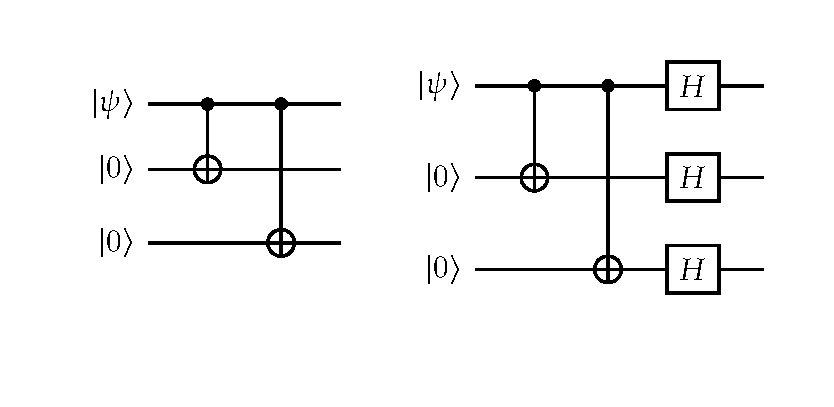
\includegraphics[width=0.8\textwidth]{Immagini/SinQuEncod.pdf}
    \caption{
        Encoder circuit for the simple single qubit error correction routines, in particular the one on the left is the one for the state flip while on the right there's the one for the phase flip.
    }
    \label{fig:SinQuEncod}
\end{figure}
The first circuit reported on the left of that figure creates a gate, that we will call $E$, that perform exactly the wanted operation. In this way the first step is performed, now we shall be able to understand if a state flip error happens by the fact that $\ket{\psi_0}$ will change state going from \eqref{eq:baseState} to one of the following
\begin{equation}
    \label{eq:FlippedStates}
    \ket{\psi_1} = a\ket{100} + b \ket{011}, \hspace{1cm} \ket{\psi_2} = a\ket{010} + b\ket{101}, \hspace{1cm} \ket{\psi_3} = a\ket{001} + b\ket{110}.
\end{equation}
The last thing that we need to understand is how we can understand in which state is the system in order to then correct it. The idea is so to mesure the state using a particular mesure defined as
\begin{align}
    &\{\hat{P}_k\}_{k=0}^3, &\hat{P}_k = \ketbra{\psi_k},
\end{align}
which will allow us to mesure exactly which state we have whithout making it collapse. In fact, if we are in a state $\ket{\psi_j}$ we will have that
\begin{equation}
    p_k = \ev{\hat{P}_k}{\psi_j} = \begin{cases}
        0 & j \neq k\\
        \abs{a}^2 + \abs{b}^2 & j = k
    \end{cases} = \delta_{jk},
\end{equation}
meaning that the only possible state in which $\ket{\psi_j}$ can collapse into is itself. This will allow us to evaluate the state perfectly giving a good diagnose of the error that has occured, a mesure that allow us to do this is called \textbf{syndrome operator}. Subsequently, after understand the state of the system, we will be able to correct the error by appling an $X$ operator on the flipped qubit.


To make an example of such measure different from the projector theoretical one, we can simply define it by using a series of $Z$ operators. We remember how $\ket{0}$ and $\ket{1}$ are the eigenstates of the operator so that $Z\ket{0/1} = +1/-1\ket{0/1}$. Knowing it we can define the operators
\begin{equation}
    Z_1Z_2 = Z_1\otimes Z_2\otimes \mathbb{1}_3 = [+1(\ketbra{00} + \ketbra{11}) -1(\ketbra{10} + \ketbra{01})]\otimes \mathbb{1}_3,
\end{equation}
which shows how it returns $+1$ if the first and second qubit are equal, and $-1$ otherwise. In this way we can define a really clever syndrome opeartor measure by using only two operators $Z_1Z_2$ and $Z_2Z_3$, having that by their value we can understand the error exactly. In fact, by knowing which qubits are equal or not allows us to tell exactly which of the four state we have in that specific moment.

This method is so an exact copy of the classical one setted in a quantum environment, and we can see how it is the same as before since the probability of an error to propagate using this routine is given exactly by \eqref{eq:ErrMajoRate}. Meaning that this can be implemented only if the error rate is already below the $50\%$, but still this is a good simple algorithm since can be applied not only to the case of the state flip but also to other type of errors. For example, for a qubit not only the state can be change by external factor, but also the phase is vulnerable. In particular, we can imagine that now the operator that is applied with a probability $p$ is $Z$, which applied on $\ket{\psi}$ will flip the phase of $\ket{1}$. One may think that such an error needs to be trated differently from the one seen before, but that would be not true. In fact, we can see how if instead of the computational base we use $\ket{\pm}$ to represent the states the problem returns to a flip of the state since $Z\ket{\pm} = \ket{\mp}$. Therefore, if we encode the states by using the circuit in \figref{fig:SinQuEncod} that performs the following tranformation
\begin{align}
    &\ket{0}\mapsto \ket{+++}, &\ket{1}\mapsto\ket{---},
\end{align}
we can then define the syndrome mesure by also changin base as the normal one and obtaining
\begin{equation}
    H^{\otimes 3} Z_1Z_2 H^{\otimes 3} = X_1X_2. 
\end{equation}
This will allow us to understand if a phase flip happens allowing us to recover the initial state without any problem, reducing the probability of error as seen before.

\subsection{Shor code}

We have seen how we are able to correct both states flips and phase flips in a separate way, but inside a quantum computer we are interested in the full correction of the qubits aiming to a protocol allowing for the correction of both at the same time. Such a routine exist and is called \textbf{Shor code} that we shall see next.

The idea starts with the encoding of the states by using a total of $9$ qubits mapping the computational base to the following monsters
\begin{align}
    &\ket{0} = \left( \frac{\ket{000} + \ket{111}}{\sqrt{2}} \right)_{B1}\left( \frac{\ket{000} + \ket{111}}{\sqrt{2}} \right)_{B2}\left( \frac{\ket{000} + \ket{111}}{\sqrt{2}} \right)_{B3} = \ket{+}_{B1}\ket{+}_{B2}\ket{+}_{B3},\\
    &\ket{1} = \left( \frac{\ket{000} - \ket{111}}{\sqrt{2}} \right)_{B1}\left( \frac{\ket{000} - \ket{111}}{\sqrt{2}} \right)_{B2}\left( \frac{\ket{000} - \ket{111}}{\sqrt{2}} \right)_{B3} = \ket{-}_{B1}\ket{-}_{B2}\ket{-}_{B3}.
\end{align}
Basically defining three blocks with inside the same encoded state of before, having in fact an encoder circuit really close to the two seen previously as depicted in \figref{fig:ShorEncoder}.
\begin{figure}[t]
    \centering
    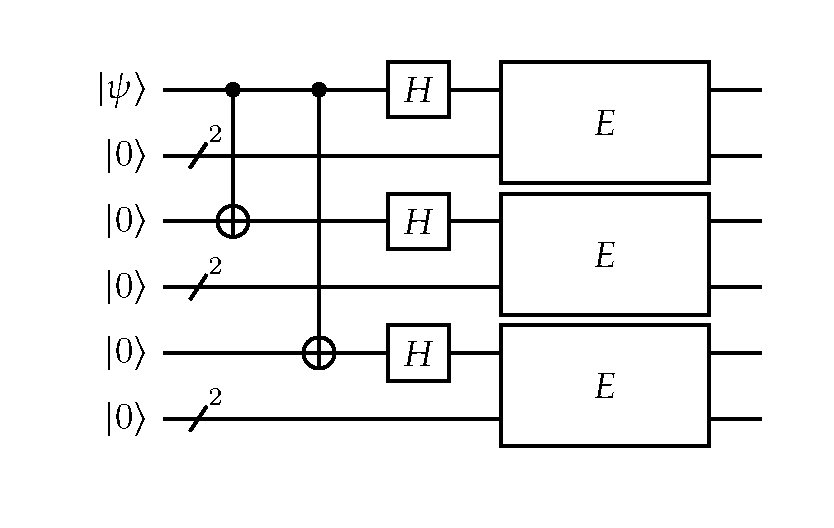
\includegraphics[width=0.8\textwidth]{Immagini/ShorEncoder.pdf}
    \caption{
        Encoder for the Shor code, where the gates defined by $E$ are ncoders for the simple case of the state flip correction.
    }
    \label{fig:ShorEncoder}
\end{figure}
Now, we can go and see what happens if we have a state or phase flip inside one of the qubit. In the case of the state flip, we can see how one of the blocks will change the state as in \eqref{eq:FlippedStates} so that we can use a generalization of the $Z_1Z_2$ measure to find out the error
\begin{equation}
    Z_1Z_2 = (Z_1Z_2)_{B1}\otimes\mathbb{1}_{B2}\otimes\mathbb{1}_{B3}.
\end{equation}
We have so an efficient way to spot the state errors and correct them by simply apply a NOT where needed. Then, for the phase flips instead we will have that one of the blocks will change having that $\ket{\pm}$ will fo into $\ket{\mp}$. To spot which one of the blocks we need to correct we can use the same idea seen previously for the phase flip, where we can use the following operators
\begin{align}
    &S_1 = X_{B1}X_{B2} = (X_1X_2X_3)\otimes(X_4X_5X_6)\otimes\mathbb{1}_{B3},\\
    &S_2 = X_{B2}X_{B3} = \mathbb{1}_{B1} \otimes (X_4X_5X_6)\otimes (X_7X_8X_9).
\end{align}
In this way we can be sure to see every possible state and phase flip inside our circuit and be able to correct them properly.
    \section{Hybrid algorithm}

In the last moment of the course the prof just introduced the concept of hybrid algorithms, which is a way of incorporating quantum routines inside classical algorithms in order to speed up computaitons. The main idea is to use quantum computers in order to evaluate complex functions inside classical algorithms, like minimization ones, since they can do it faster.

Therefore, I will write down the simple example that she showed during class and stop there, since the course has effectivelly stopped at that moment.

\subsection{Quantum Approximation Optimizzation Algorithm}

The idea is that we want to minimize the energy of a system finding the ground state of a Hamiltonian $\hat{\mathcal{H}}_c$. To do that an ansatz for the GS $\ket{\psi}$ is created depending on some parameters $\ket{\psi(\vb*{\theta})}$ and the set $\vb*{\theta}_0$ that minimize the function
\begin{equation}
    f(\vb*{\theta}) = \ev{\hat{\mathcal{H}}_c}{\psi(\vb*{\theta})},
\end{equation}
is found out by minimization. What we want to do is evaluate $f$ by using quantum algorithm and find the minimum using the classical approach since QC still are not good at it. Therefore, the general outline of the algorithm should be the following:
\begin{enumerate}[label*=\protect\fbox{\arabic{enumi}}]
    \item Prepare the ansatz $\ket{\psi(\theta)}$ through the use of a series of operator $\{\mathcal{U}_{\theta_1}, \mathcal{U}_{\theta_2}, \dots, \mathcal{U}_{\theta_p}\}$, where $p$ is called depth of the algorithm;
    \item Use $\hat{\mathcal{H}}_c$ to measure the state obtained state $\ket{\psi(\vb*{\theta})}$ $N$ times, so that every time we will obtain a different weigenvalue $E_\lambda$ with probability $p_\lambda$ that we can use to approximate $f$ as follws
    \begin{equation}
        \label{eq:QuantumApproxF}
        f(\vb*{\theta}) = \sum_\lambda E_\lambda p_\lambda \approx \sum_\lambda E_\lambda \frac{n_\lambda}{N}.    
    \end{equation} 
    \item Pass the result to the classical computer to perform the minimization algorithm.
\end{enumerate}
One can easily understand how perform the computation \eqref{eq:QuantumApproxF} is able to approximate the value of $f$ in a sufficiently accurate way that is easier to achive than perform the integration of the high dimensional $\ket{\psi}$. Such an algorithm seems already good to work, but in reality problems are present on both first and third point of the whole construction. We will focus on the first step since it's more interesting as a problem how to effectivelly construct the $\mathcal{U}_{\theta}$ operators, and we will only give a glimps of the problem in the third point.

To construct the ansatz the main approach used is to work with evolution in the space of parameters guided by two Hamiltonians $\hat{\mathcal{H}}_1$ and $\hat{\mathcal{H}}_2$ so that the operators can be written as 
\begin{equation}
    \mathcal{U}_{\theta_i} = e^{i\theta_i\hat{\mathcal{H}}_1}e^{i\theta_{i+1}\hat{\mathcal{H}}_2},
\end{equation}
meaning that now, the parameters grows from $p$ to $2p$. Using this forms allows for a good mobility inside the state space only if the two operators are not close togheter, meaning that if $\hat{\mathcal{H}}_1 = \lambda\hat{\mathcal{H}}_2$ a problemwould occur since the evolution will only span the state of $\hat{\mathcal{H}}_1$ and all the possible ones. For this reason we need to  take Hamiltonians that are different from each other's having
\begin{equation}
    \left[ \hat{\mathcal{H}}_1, \hat{\mathcal{H}}_2 \right] \neq 0.
\end{equation}
That is a requirement, but it's not sad that is the only one needed but still we don't know for certain, as we don't know if exist a possible best choice for the two operator in order to arrive at the result quicker than all the others way. Nevertheless, what we can do now is show the main tricks tha tare used in order to construct the state:
\begin{itemize}[align=left, leftmargin=*]
    \item[\textbf{Trotler.}] One possible situation is when we have $\hat{\mathcal{H}}_c = \hat{\mathcal{H}}_1 + \hat{\mathcal{H}}_2$ with the two pieces that do not commute. In that case we can use the Trotler result in order to approximate the evolution that brings to the ground state as
    \begin{equation}
        e^{it\hat{\mathcal{H}}_c} \approx \left( e^{i\epsilon\hat{\mathcal{H}}_1}e^{i\epsilon\hat{\mathcal{H}}_2} \right)^N.
    \end{equation}
    \item[\textbf{Exact Hamiltonian.}] In the case we know the exact Hamiltonian of the system is quite helpfull instead of going trotler using it so that $\hat{\mathcal{H}}_1 = \hat{\mathcal{H}}_c$ and choose the second simply in order to not commute.
\end{itemize}
In both ways we should have at the end a series of operations that can span all the phase space depending on the paramters $\vb*{\theta}$ that needs to be optimized. And the problem in the third point is exactly there, the optimization of $\vb*{\theta}$ is a pain for several reasons. The main problem is that the energetic landscape inside parameter space looks really like a plateu with a big minimum in a certain point, is just like that we need to accept that. Nevertheless, such a situation is a complicated one since means that $\grad_{\vb*{\theta}} f(\vb*{\theta}) \approx 0$ in a wide range. Therefore, the simple gradient descend method can't be used efficiently we need more complex algorithms but find the right one is a challenge that we are still facing.
\ex{Maximal independent set}
{
    At a last the prof made a simple example of minimization problem that can be tackled using those hybrid algorithms. The problem is to find out a particular set of nodes inside a network and to do that you describe the nodes using a state like
    \begin{equation}
        \ket{0110011\dots},
    \end{equation}
    where every qubit rapresent a specific node and $1$ means that are in the wanted set, while $0$ otherwise. The only thing that remains to do is to engenier a Hamiltonian that has the right state as the gorund state, but that can be done by using an appropriate Ising model
    \begin{align}
        &\hat{\mathcal{H}}_c = \sum_i Z_i + P\sum_{\langle ij \rangle} Z_iZ_j, &f_c = \ev{\hat{\mathcal{H}}_c}{\psi}.
    \end{align}
    In this way you only need to decide the right nearest negihbours and the value of the penalty $P$ to obtain the wanted result. Also, this approch allows for the use of the second kind of approach to create the ansatz really easily by using as $\hat{\mathcal{H}}_1 = \hat{\mathcal{H}}_c$ and $\hat{\mathcal{H}}_2 = \sum_i X_i$ that usually can make the algorithm efficient.
}
\nt
{
    It's interesting to understand also how in the approach described for the creation of the ansatz it's obvius that we will have only an approximation of the expected $\ket{\psi(\vb*{\theta})}$ state, but still that is not a problem. In fact, one can see how defining the fidelity of the procedure as
    \begin{displaymath}
        Fid = \braket{\psi_{exact}}{\psi(\vb*{\theta})},
    \end{displaymath}
    we have that a fidelity fo $0.8$ is already good to have values of energies precise up to six or seven decimals since the energy converges much faster thatn the eigenstate.
}

    % \chapter{Exercises}
    % \section{Gates}

\qs{Double control gate}
{
    Verify the equivalence of the two following circuits:
    \begin{center}
        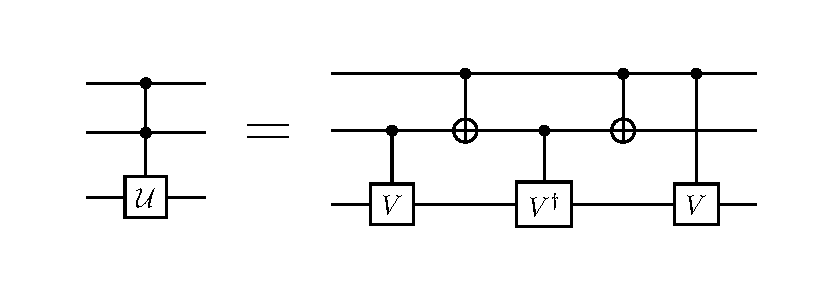
\includegraphics[width=0.7\textwidth]{Immagini/CCU.pdf}
    \end{center}
    Where the unitary operation $V$ is defined as $\sqrt{\mathcal{U}}$.
}
\pf{Solution}
{
    Two main ways of soliving this problem can be used, the first and simplest one is by constructing the thruth table of the two circuits and see that is the same. Something that is left to the reader since it's a really simple task. The other one is by going with a matrix multiplication and seing how the matrix form of the circuit on the right is the same as the general double control. To see that first we can write the following form of the matrix of the circuit
    \begin{equation}
        \left( CV_{13}\otimes\mathbb{1}_2 \right)\left( CNOT_{12}\otimes \mathbb{1}_3 \right)\left( \mathbb{1}_1\otimes CV^\dagger_{23} \right)\left( CNOT_{12}\otimes \mathbb{1}_3 \right)\left( \mathbb{1}_1 \otimes CV_{23} \right).
    \end{equation}
    Now, we know how to write down the majority of those matrices but one. For example, we can easily write the following thing
    \begin{equation}
        \mathbb{1}_1\otimes CV^\dagger_{23} = \begin{pmatrix}
            1 & 0\\
            0 & 1
        \end{pmatrix}\otimes\begin{pmatrix}
            \mathbb{1} & \mathbb{0}\\
            \mathbb{0} & V
        \end{pmatrix} = \begin{pmatrix}
            \mathbb{1} & \mathbb{0} & \mathbb{0} & \mathbb{0}\\
            \mathbb{0} & V & \mathbb{0} & \mathbb{0}\\
            \mathbb{0} & \mathbb{0} & \mathbb{1} & \mathbb{0}\\
            \mathbb{0} & \mathbb{0} & \mathbb{0} & V\\
        \end{pmatrix},
    \end{equation}
    where the tensor product rule has been used in the multiplication. Still, a problem is present in the evaluation of the first matrix, because the order matters in tensor product and in that case the control is applied to a qubit that is not directly attached to the one of the target. Therefore, the main way we have to evaluate that matrix is to swap the qubit and then use a normal control gate as we have seen right now
    \begin{equation}
        CV_{13}\otimes\mathbb{1}_2 = \left( S_{12}\otimes\mathbb{1}_3 \right)\left( \mathbb{1}_1 \otimes CV_{23} \right)\left( S_{12}\otimes\mathbb{1}_3 \right).
    \end{equation}
    By recalling the form of the swap operator matrix being \eqref{eq:swapMatrix} we can perform now all the computation to obtain
    \begin{equation}
        CV_{13}\otimes\mathbb{1}_2 = \begin{pmatrix}
            \mathbb{1} & \mathbb{0} & \mathbb{0} & \mathbb{0}\\
            \mathbb{0} & \mathbb{1} & \mathbb{0} & \mathbb{0}\\
            \mathbb{0} & \mathbb{0} & V & \mathbb{0}\\
            \mathbb{0} & \mathbb{0} & \mathbb{0} & V\\
        \end{pmatrix},
    \end{equation}
    which then can be used to perform the matrix multiplication and obtain the final form of the gate that wuold be analogous to the one of a CCU gate.
}
    % \section{Measure}

\qs{General one qubit measure}
{
    Take the general form of an observable acting on a qubit $A = \vb{n}\vdot\vb*{\sigma}$, where $\vb*{\sigma}$ is a vector containing the Pauli matrices and $\vb{n}$ is real versor. Find out the possible outcomes of a measure done on a general state $\ket{\psi}$ and their probability of happening.

    At last, show how the measuring $A$ on the computational basis is not totally equivalent to measuring it in the $\ket{e_\pm}$ orthonormal base of eigenstates since $\ket{\psi}$ collapse in different states, but the following circuit
    \begin{center}
        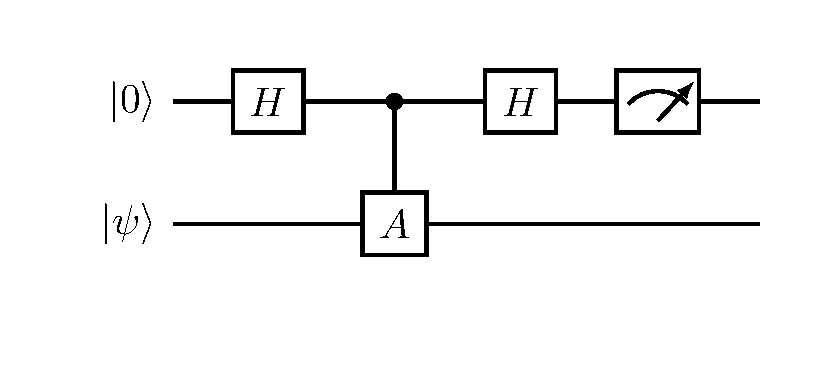
\includegraphics[width=0.7\textwidth]{Immagini/POVM.pdf}
    \end{center}
    can instead reproduce the exact measure by evaluating the axiliary qubit, forming the POVM of the $A$ PVM measure.
}
\pf{Solution}
{
    First we can easily find out the values of the eigenvalues by using the following trick. We can take the square of the matrix seeing how
    \begin{equation}
        \left( \vb{n}\vdot\vb*{\sigma} \right)^2 = n_x^2 X^2 + n_y^2 Y^2 + n_z^2Z^2 + n_xn_yXY + n_xn_yYX + \dots,
    \end{equation}
    by recalling that $XY = -YX$ for every couple of Pauli matrix and $X^2=Y^2=Z^2 = \mathbb{1}$ we can see how
    \begin{equation}
        \left( \vb{n}\vdot\vb*{\sigma} \right)^2 = \abs{\vb{n}}\mathbb{1} = \mathbb{1}.
    \end{equation}
    Therefore, we can say that the squares of the eigenvalues of $A$ needs to give $1$, but we can also say that the following is true
    \begin{equation}
        \trace{A} = n_x \trace{X} + n_y \trace{Y} + n_z\trace{Z} = 0.
    \end{equation}
    Meaning that we can now find out the eigenvalues of the matrix $\lambda_{\pm}$ simply by knowing that $\abs{\lambda_{\pm}}^2 = 1$ and that their sum needs to be zero $\lambda_+ + \lambda_- = 0$ having that the only possible solution is
    \begin{align}
        &\lambda_+ = +1, &\lambda_- = -1.
    \end{align}
    Meaning that the only possible outcomes of the measure is still $\pm 1$ also for this observable.

    Now, to measure the probability of one outcome to appear we need to write down the projector on the base of the observable. In particular, we can say that being $A$ selfadjoint a base $\ket{e_\pm}$ of eigenvector exist whose projectors $P_\pm = \ketbra{e_{\pm}}$ has the properties
    \begin{align}
        &\vb{n}\vdot\vb*{\sigma} = P_+ - P_-, &\mathbb{1} = P_+ + P_-.
    \end{align}
    Meaning that we can invert those and find out in the end the following forms
    \begin{equation}
        P_\pm = \frac{\mathbb{1} \pm A}{2}.
    \end{equation}
    From this we can easily write down the probabilities of measuring in a state like $\ket{\psi} = \alpha\ket{e_+} + \beta\ket{e_2}$ which are simply $p_+ = \abs{\alpha}^2$ and $p_- = \abs{\beta}^2$. Nevertheless, we are interested also in evaluating it in the computational base so that the state is written as  $\ket{\psi} = a\ket{0} + b\ket{1}$ having that the probability becomes
    \begin{equation}
        \tilde{p}_\pm = \ev{P_\pm}{\psi} = \frac{1}{2}\left[ (1\pm n_z) \pm 2n_x\Re{a^*b} \pm 2n_y\Im{a^*b} \right].
    \end{equation}
    Where one can see how the coefficients generate added terms to the probabilities in case of superpositioning, meaning that if one of the two $a$ or $b$ is zero the added terms vanishes. Also, those terms depends on the relative phase of the two coeffiecients meaning that \textbf{interference effects} can happen. Still, the values obtained are in reality equal to the one of $\alpha$ and $\beta$ squared seen previusly if one does all the computations, meaning that the probabilities evaluated in the two bases are the same. What changes is the collapsing since in the normal base $\ket{\psi}$ collapse in one of the two $\ket{e_\pm}$ while in the computational will become either $\ket{0}$ or $\ket{1}$.

    We can now see how the circuit we have seen that uses an auxiliary qubit to perform the computation is able to generate the exact measure we are searching for, also forming a POVM for that measure. To see that we can see how the state of the system evolves inside the circuit by starting from the application of the Hadamert gate and of the CA one having
    \begin{equation}
        \ket{0}\ket{\psi} = \frac{\ket{0}\ket{\psi} + \ket{1}A\ket{\psi}}{\sqrt{2}}.
    \end{equation}
    Then, by using a second Hadamart gate we can easily see how the state can be written simply as
    \begin{equation}
        \ket{0}\left( \frac{\mathbb{1} + A}{2} \right)\ket{\psi} + \ket{1}\left( \frac{\mathbb{1} - A}{2} \right)\ket{\psi} = \ket{0}P_+\ket{\psi} + \ket{1}P_-\ket{\psi}.
    \end{equation}
    Meaning that we have an entangled state where, by measuring the first qubit in the computational base allow us to know the state of $\ket{\psi}$ that has collapsed in one of the two eigenstate of $A$. Also, we can see how the probability of measuring the outcome $\pm 1$ in the computational base is given by
    \begin{equation}
        \braket{0}\ev{P_\pm^\dagger P_\pm}{\psi} = \tilde{p}_\pm.
    \end{equation}
    Basically the probabilities remains the same but now the states collapse in the right way so that the full measure is obtained, we only need one extra qubit.
}

\end{document}